\documentclass[twoside]{book}

% Packages required by doxygen
\usepackage{fixltx2e}
\usepackage{calc}
\usepackage{doxygen}
\usepackage[export]{adjustbox} % also loads graphicx
\usepackage{graphicx}
\usepackage[utf8]{inputenc}
\usepackage{makeidx}
\usepackage{multicol}
\usepackage{multirow}
\PassOptionsToPackage{warn}{textcomp}
\usepackage{textcomp}
\usepackage[nointegrals]{wasysym}
\usepackage[table]{xcolor}

% Font selection
\usepackage[T1]{fontenc}
\usepackage[scaled=.90]{helvet}
\usepackage{courier}
\usepackage{amssymb}
\usepackage{sectsty}
\renewcommand{\familydefault}{\sfdefault}
\allsectionsfont{%
  \fontseries{bc}\selectfont%
  \color{darkgray}%
}
\renewcommand{\DoxyLabelFont}{%
  \fontseries{bc}\selectfont%
  \color{darkgray}%
}
\newcommand{\+}{\discretionary{\mbox{\scriptsize$\hookleftarrow$}}{}{}}

% Page & text layout
\usepackage{geometry}
\geometry{%
  a4paper,%
  top=2.5cm,%
  bottom=2.5cm,%
  left=2.5cm,%
  right=2.5cm%
}
\tolerance=750
\hfuzz=15pt
\hbadness=750
\setlength{\emergencystretch}{15pt}
\setlength{\parindent}{0cm}
\setlength{\parskip}{3ex plus 2ex minus 2ex}
\makeatletter
\renewcommand{\paragraph}{%
  \@startsection{paragraph}{4}{0ex}{-1.0ex}{1.0ex}{%
    \normalfont\normalsize\bfseries\SS@parafont%
  }%
}
\renewcommand{\subparagraph}{%
  \@startsection{subparagraph}{5}{0ex}{-1.0ex}{1.0ex}{%
    \normalfont\normalsize\bfseries\SS@subparafont%
  }%
}
\makeatother

% Headers & footers
\usepackage{fancyhdr}
\pagestyle{fancyplain}
\fancyhead[LE]{\fancyplain{}{\bfseries\thepage}}
\fancyhead[CE]{\fancyplain{}{}}
\fancyhead[RE]{\fancyplain{}{\bfseries\leftmark}}
\fancyhead[LO]{\fancyplain{}{\bfseries\rightmark}}
\fancyhead[CO]{\fancyplain{}{}}
\fancyhead[RO]{\fancyplain{}{\bfseries\thepage}}
\fancyfoot[LE]{\fancyplain{}{}}
\fancyfoot[CE]{\fancyplain{}{}}
\fancyfoot[RE]{\fancyplain{}{\bfseries\scriptsize Generated by Doxygen }}
\fancyfoot[LO]{\fancyplain{}{\bfseries\scriptsize Generated by Doxygen }}
\fancyfoot[CO]{\fancyplain{}{}}
\fancyfoot[RO]{\fancyplain{}{}}
\renewcommand{\footrulewidth}{0.4pt}
\renewcommand{\chaptermark}[1]{%
  \markboth{#1}{}%
}
\renewcommand{\sectionmark}[1]{%
  \markright{\thesection\ #1}%
}

% Indices & bibliography
\usepackage{natbib}
\usepackage[titles]{tocloft}
\setcounter{tocdepth}{3}
\setcounter{secnumdepth}{5}
\makeindex

% Hyperlinks (required, but should be loaded last)
\usepackage{ifpdf}
\ifpdf
  \usepackage[pdftex,pagebackref=true]{hyperref}
\else
  \usepackage[ps2pdf,pagebackref=true]{hyperref}
\fi
\hypersetup{%
  colorlinks=true,%
  linkcolor=blue,%
  citecolor=blue,%
  unicode%
}

% Custom commands
\newcommand{\clearemptydoublepage}{%
  \newpage{\pagestyle{empty}\cleardoublepage}%
}

\usepackage{caption}
\captionsetup{labelsep=space,justification=centering,font={bf},singlelinecheck=off,skip=4pt,position=top}

%===== C O N T E N T S =====

\begin{document}

% Titlepage & ToC
\hypersetup{pageanchor=false,
             bookmarksnumbered=true,
             pdfencoding=unicode
            }
\pagenumbering{alph}
\begin{titlepage}
\vspace*{7cm}
\begin{center}%
{\Large Lander simulation }\\
\vspace*{1cm}
{\large Generated by Doxygen 1.8.13}\\
\end{center}
\end{titlepage}
\clearemptydoublepage
\pagenumbering{roman}
\tableofcontents
\clearemptydoublepage
\pagenumbering{arabic}
\hypersetup{pageanchor=true}

%--- Begin generated contents ---
\chapter{CS 5201 Assignment 5}
\label{md_README}
\Hypertarget{md_README}
Read the directions on the \href{https://jberm6.git-pages.mst.edu/essman/homework/hw5/}{\tt course website}

\subsubsection*{Automated Tests}

You have been provided with a small subset of the tests that your code will be subjected to. This is not a substitute for writing your own tests. To run your tests locally, simply {\ttfamily cd tests} and then execute {\ttfamily ./test\+\_\+main.sh}. Your tests will also be executed when you push to Git\+Lab. Do not modify the tests or any of the relevant files. Doing so will be treated like any other act of academic dishonesty. You should, however, modify {\ttfamily my\+Matrix\+Name.\+txt}, to include the name of your vector class. If the contents of this file are {\ttfamily my\+Matrix}, the grading script will assume that you have a header file called {\ttfamily my\+Matrix.\+h} which contains the declaration of a class called {\ttfamily my\+Matrix}. 
\chapter{Hierarchical Index}
\section{Class Hierarchy}
This inheritance list is sorted roughly, but not completely, alphabetically\+:\begin{DoxyCompactList}
\item \contentsline{section}{filter$<$ T $>$}{\pageref{classfilter}}{}
\begin{DoxyCompactList}
\item \contentsline{section}{dummy$<$ T $>$}{\pageref{classdummy}}{}
\item \contentsline{section}{kalman$<$ T $>$}{\pageref{classkalman}}{}
\item \contentsline{section}{low\+Pass$<$ T $>$}{\pageref{classlowPass}}{}
\end{DoxyCompactList}
\item \contentsline{section}{n\+Vect$<$ T $>$\+:\+:iterator}{\pageref{classnVect_1_1iterator}}{}
\item \contentsline{section}{lander}{\pageref{classlander}}{}
\item \contentsline{section}{n\+Trix$<$ T $>$}{\pageref{classnTrix}}{}
\item \contentsline{section}{n\+Vect$<$ T $>$}{\pageref{classnVect}}{}
\item \contentsline{section}{n\+Vect$<$ float $>$}{\pageref{classnVect}}{}
\item \contentsline{section}{P\+ID}{\pageref{classPID}}{}
\end{DoxyCompactList}

\chapter{Class Index}
\section{Class List}
Here are the classes, structs, unions and interfaces with brief descriptions\+:\begin{DoxyCompactList}
\item\contentsline{section}{\hyperlink{classdummy}{dummy$<$ T $>$} \\*Dummy class }{\pageref{classdummy}}{}
\item\contentsline{section}{\hyperlink{classfilter}{filter$<$ T $>$} \\*Filter class }{\pageref{classfilter}}{}
\item\contentsline{section}{\hyperlink{classnVect_1_1iterator}{n\+Vect$<$ T $>$\+::iterator} \\*Iterator class }{\pageref{classnVect_1_1iterator}}{}
\item\contentsline{section}{\hyperlink{classkalman}{kalman$<$ T $>$} \\*Kalman class }{\pageref{classkalman}}{}
\item\contentsline{section}{\hyperlink{classlander}{lander} \\*Lander class }{\pageref{classlander}}{}
\item\contentsline{section}{\hyperlink{classlowPass}{low\+Pass$<$ T $>$} \\*Low\+Pass class }{\pageref{classlowPass}}{}
\item\contentsline{section}{\hyperlink{classnTrix}{n\+Trix$<$ T $>$} \\*N\+Trix class }{\pageref{classnTrix}}{}
\item\contentsline{section}{\hyperlink{classnVect}{n\+Vect$<$ T $>$} \\*N\+Vect class }{\pageref{classnVect}}{}
\item\contentsline{section}{\hyperlink{classPID}{P\+ID} \\*\hyperlink{classPID}{P\+ID} class }{\pageref{classPID}}{}
\end{DoxyCompactList}

\chapter{File Index}
\section{File List}
Here is a list of all documented files with brief descriptions\+:\begin{DoxyCompactList}
\item\contentsline{section}{\hyperlink{dummy_8h}{dummy.\+h} }{\pageref{dummy_8h}}{}
\item\contentsline{section}{{\bfseries dummy.\+hpp} }{\pageref{dummy_8hpp}}{}
\item\contentsline{section}{\hyperlink{filter_8h}{filter.\+h} }{\pageref{filter_8h}}{}
\item\contentsline{section}{\hyperlink{kalman_8h}{kalman.\+h} }{\pageref{kalman_8h}}{}
\item\contentsline{section}{{\bfseries kalman.\+hpp} }{\pageref{kalman_8hpp}}{}
\item\contentsline{section}{\hyperlink{lander_8h}{lander.\+h} }{\pageref{lander_8h}}{}
\item\contentsline{section}{{\bfseries lander.\+hpp} }{\pageref{lander_8hpp}}{}
\item\contentsline{section}{\hyperlink{lowPass_8h}{low\+Pass.\+h} }{\pageref{lowPass_8h}}{}
\item\contentsline{section}{{\bfseries low\+Pass.\+hpp} }{\pageref{lowPass_8hpp}}{}
\item\contentsline{section}{\hyperlink{nTrix_8h}{n\+Trix.\+h} }{\pageref{nTrix_8h}}{}
\item\contentsline{section}{{\bfseries n\+Trix.\+hpp} }{\pageref{nTrix_8hpp}}{}
\item\contentsline{section}{\hyperlink{nVect_8h}{n\+Vect.\+h} }{\pageref{nVect_8h}}{}
\item\contentsline{section}{{\bfseries n\+Vect.\+hpp} }{\pageref{nVect_8hpp}}{}
\item\contentsline{section}{\hyperlink{PID_8h}{P\+I\+D.\+h} }{\pageref{PID_8h}}{}
\end{DoxyCompactList}

\chapter{Class Documentation}
\hypertarget{classdummy}{}\section{dummy$<$ T $>$ Class Template Reference}
\label{classdummy}\index{dummy$<$ T $>$@{dummy$<$ T $>$}}


dummy class.  




{\ttfamily \#include $<$dummy.\+h$>$}



Inheritance diagram for dummy$<$ T $>$\+:\nopagebreak
\begin{figure}[H]
\begin{center}
\leavevmode
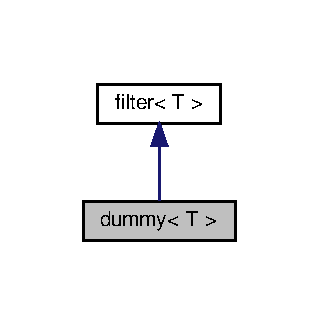
\includegraphics[width=153pt]{classdummy__inherit__graph}
\end{center}
\end{figure}


Collaboration diagram for dummy$<$ T $>$\+:\nopagebreak
\begin{figure}[H]
\begin{center}
\leavevmode
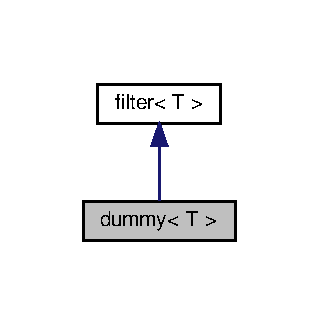
\includegraphics[width=153pt]{classdummy__coll__graph}
\end{center}
\end{figure}
\subsection*{Public Member Functions}
\begin{DoxyCompactItemize}
\item 
virtual \hyperlink{classnVect}{n\+Vect}$<$ T $>$ \hyperlink{classdummy_a437aae6ce48cad80944cb578aa0c0218}{operator()} (\hyperlink{classnVect}{n\+Vect}$<$ T $>$ \&state)
\begin{DoxyCompactList}\small\item\em () operator \end{DoxyCompactList}\end{DoxyCompactItemize}


\subsection{Detailed Description}
\subsubsection*{template$<$typename T$>$\newline
class dummy$<$ T $>$}

dummy class. 

This class is a derived filter class that acts as a passthrough of a state without actually filtering it. 

\subsection{Member Function Documentation}
\mbox{\Hypertarget{classdummy_a437aae6ce48cad80944cb578aa0c0218}\label{classdummy_a437aae6ce48cad80944cb578aa0c0218}} 
\index{dummy@{dummy}!operator()@{operator()}}
\index{operator()@{operator()}!dummy@{dummy}}
\subsubsection{\texorpdfstring{operator()()}{operator()()}}
{\footnotesize\ttfamily template$<$typename T $>$ \\
\hyperlink{classnVect}{n\+Vect}$<$ T $>$ \hyperlink{classdummy}{dummy}$<$ T $>$\+::operator() (\begin{DoxyParamCaption}\item[{\hyperlink{classnVect}{n\+Vect}$<$ T $>$ \&}]{state }\end{DoxyParamCaption})\hspace{0.3cm}{\ttfamily [virtual]}}



() operator 

Description\+: () operator overload that inherits from the base class to allow the user to pass a n\+Vect$<$\+T$>$ state through. 
\begin{DoxyParams}{Parameters}
{\em state} & is the state that the user wants to pass through unfiltered. \\
\hline
\end{DoxyParams}
\begin{DoxyReturn}{Returns}
Returns a new n\+Vect$<$\+T$>$ that has the same values as the parameter. 
\end{DoxyReturn}


Implements \hyperlink{classfilter_ac8ec0fb4a10d10ee5e3133259610e0d2}{filter$<$ T $>$}.



The documentation for this class was generated from the following files\+:\begin{DoxyCompactItemize}
\item 
\hyperlink{dummy_8h}{dummy.\+h}\item 
dummy.\+hpp\end{DoxyCompactItemize}

\hypertarget{classfilter}{}\section{filter$<$ T $>$ Class Template Reference}
\label{classfilter}\index{filter$<$ T $>$@{filter$<$ T $>$}}


filter class.  




{\ttfamily \#include $<$filter.\+h$>$}



Inheritance diagram for filter$<$ T $>$\+:\nopagebreak
\begin{figure}[H]
\begin{center}
\leavevmode
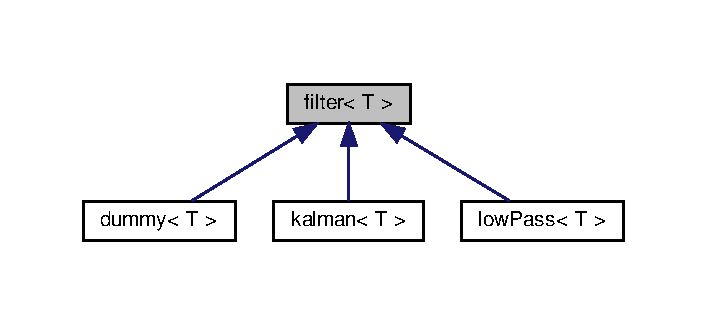
\includegraphics[width=340pt]{classfilter__inherit__graph}
\end{center}
\end{figure}
\subsection*{Public Member Functions}
\begin{DoxyCompactItemize}
\item 
virtual \hyperlink{classnVect}{n\+Vect}$<$ T $>$ \hyperlink{classfilter_ac8ec0fb4a10d10ee5e3133259610e0d2}{operator()} (\hyperlink{classnVect}{n\+Vect}$<$ T $>$ \&state)=0
\begin{DoxyCompactList}\small\item\em () operator \end{DoxyCompactList}\end{DoxyCompactItemize}


\subsection{Detailed Description}
\subsubsection*{template$<$typename T$>$\newline
class filter$<$ T $>$}

filter class. 

This class is a base filter class that allows the user to specify derived filter classes with () functionality. 

\subsection{Member Function Documentation}
\mbox{\Hypertarget{classfilter_ac8ec0fb4a10d10ee5e3133259610e0d2}\label{classfilter_ac8ec0fb4a10d10ee5e3133259610e0d2}} 
\index{filter@{filter}!operator()@{operator()}}
\index{operator()@{operator()}!filter@{filter}}
\subsubsection{\texorpdfstring{operator()()}{operator()()}}
{\footnotesize\ttfamily template$<$typename T $>$ \\
virtual \hyperlink{classnVect}{n\+Vect}$<$T$>$ \hyperlink{classfilter}{filter}$<$ T $>$\+::operator() (\begin{DoxyParamCaption}\item[{\hyperlink{classnVect}{n\+Vect}$<$ T $>$ \&}]{state }\end{DoxyParamCaption})\hspace{0.3cm}{\ttfamily [pure virtual]}}



() operator 

Description\+: () operator overload for the filter base class. Allows the user to access the () operator functionality of a derived class through the base class. 
\begin{DoxyParams}{Parameters}
{\em state} & is a n\+Vect$<$\+T$>$ object that the filter takes in to filter. \\
\hline
\end{DoxyParams}
\begin{DoxyReturn}{Returns}
Returns a n\+Vect$<$\+T$>$ which represents the filtered state. 
\end{DoxyReturn}


Implemented in \hyperlink{classkalman_ae3c0c97ba8c3eb2eba0134a3adf701ed}{kalman$<$ T $>$}, \hyperlink{classlowPass_a4d4458814fd69f87c5622227f6527468}{low\+Pass$<$ T $>$}, and \hyperlink{classdummy_a437aae6ce48cad80944cb578aa0c0218}{dummy$<$ T $>$}.



The documentation for this class was generated from the following file\+:\begin{DoxyCompactItemize}
\item 
\hyperlink{filter_8h}{filter.\+h}\end{DoxyCompactItemize}

\hypertarget{classnVect_1_1iterator}{}\section{n\+Vect$<$ T $>$\+:\+:iterator Class Reference}
\label{classnVect_1_1iterator}\index{n\+Vect$<$ T $>$\+::iterator@{n\+Vect$<$ T $>$\+::iterator}}


iterator class.  




{\ttfamily \#include $<$n\+Vect.\+h$>$}

\subsection*{Public Member Functions}
\begin{DoxyCompactItemize}
\item 
\hyperlink{classnVect_1_1iterator_a8e19f7baeffbc2b8320f4b530be16d86}{iterator} (\hyperlink{classnVect}{n\+Vect}$<$ T $>$ $\ast$a, unsigned int idx)
\begin{DoxyCompactList}\small\item\em constructor \end{DoxyCompactList}\item 
T \& \hyperlink{classnVect_1_1iterator_a03ab1ec9dbcf379a4c0723536d763306}{operator$\ast$} ()
\begin{DoxyCompactList}\small\item\em 
\begin{DoxyItemize}
\item operator 
\end{DoxyItemize}\end{DoxyCompactList}\item 
T \& \hyperlink{classnVect_1_1iterator_a58333e36f3e8bc4519b41667dbf4a710}{operator-\/$>$} ()
\begin{DoxyCompactList}\small\item\em -\/$>$ operator \end{DoxyCompactList}\item 
\hyperlink{classnVect_1_1iterator}{iterator} \& \hyperlink{classnVect_1_1iterator_a92ca21ca2cc2d12095cafccf7c0d1e8f}{operator++} ()
\begin{DoxyCompactList}\small\item\em operator ++ (postfix) \end{DoxyCompactList}\item 
\hyperlink{classnVect_1_1iterator}{iterator} \hyperlink{classnVect_1_1iterator_aa77cebd3d9132f8490609d9522be8b26}{operator++} (int)
\begin{DoxyCompactList}\small\item\em operator ++ (prefix) \end{DoxyCompactList}\item 
\hyperlink{classnVect_1_1iterator}{iterator} \& \hyperlink{classnVect_1_1iterator_abece3b68bb91a0397f58bbdac7996724}{operator+=} (const unsigned int inc)
\begin{DoxyCompactList}\small\item\em += operator \end{DoxyCompactList}\item 
\hyperlink{classnVect_1_1iterator}{iterator} \& \hyperlink{classnVect_1_1iterator_a65e426d74204084e00d8d6770b88b790}{operator-\/-\/} ()
\begin{DoxyCompactList}\small\item\em operator -- (postfix) \end{DoxyCompactList}\item 
\hyperlink{classnVect_1_1iterator}{iterator} \hyperlink{classnVect_1_1iterator_aa99d3a05bc566f235dcc06c3b57e21d3}{operator-\/-\/} (int)
\begin{DoxyCompactList}\small\item\em operator -- (prefix) \end{DoxyCompactList}\item 
\hyperlink{classnVect_1_1iterator}{iterator} \& \hyperlink{classnVect_1_1iterator_a1dc00f521ea60257023cd95a1e9238dd}{operator-\/=} (const unsigned int dec)
\begin{DoxyCompactList}\small\item\em -\/= operator \end{DoxyCompactList}\end{DoxyCompactItemize}
\subsection*{Friends}
\begin{DoxyCompactItemize}
\item 
bool \hyperlink{classnVect_1_1iterator_a81d10d7799462c7ca5e7cf19119ca356}{operator==} (const \hyperlink{classnVect_1_1iterator}{iterator} \&a, const \hyperlink{classnVect_1_1iterator}{iterator} \&b)
\begin{DoxyCompactList}\small\item\em == operator \end{DoxyCompactList}\item 
bool \hyperlink{classnVect_1_1iterator_a55a8ee0e80dad1a7da9d751c25bc0386}{operator!=} (const \hyperlink{classnVect_1_1iterator}{iterator} \&a, const \hyperlink{classnVect_1_1iterator}{iterator} \&b)
\begin{DoxyCompactList}\small\item\em != operator \end{DoxyCompactList}\end{DoxyCompactItemize}


\subsection{Detailed Description}
\subsubsection*{template$<$typename T$>$\newline
class n\+Vect$<$ T $>$\+::iterator}

iterator class. 

This class allows for iterating over the \hyperlink{classnVect}{n\+Vect} object containers. 

\subsection{Constructor \& Destructor Documentation}
\mbox{\Hypertarget{classnVect_1_1iterator_a8e19f7baeffbc2b8320f4b530be16d86}\label{classnVect_1_1iterator_a8e19f7baeffbc2b8320f4b530be16d86}} 
\index{n\+Vect\+::iterator@{n\+Vect\+::iterator}!iterator@{iterator}}
\index{iterator@{iterator}!n\+Vect\+::iterator@{n\+Vect\+::iterator}}
\subsubsection{\texorpdfstring{iterator()}{iterator()}}
{\footnotesize\ttfamily template$<$typename T$>$ \\
\hyperlink{classnVect}{n\+Vect}$<$ T $>$\+::iterator\+::iterator (\begin{DoxyParamCaption}\item[{\hyperlink{classnVect}{n\+Vect}$<$ T $>$ $\ast$}]{a,  }\item[{unsigned int}]{idx }\end{DoxyParamCaption})\hspace{0.3cm}{\ttfamily [inline]}}



constructor 

Description\+: Constructs an iterator over a certain \hyperlink{classnVect}{n\+Vect} object starting at a specified integer. 
\begin{DoxyParams}{Parameters}
{\em a} & is the pointer to a \hyperlink{classnVect}{n\+Vect} to be copied. \\
\hline
{\em idx} & is the index position of the pointer. \\
\hline
\end{DoxyParams}
\begin{DoxyPostcond}{Postcondition}
Creates a new iterator object with the specified data. 
\end{DoxyPostcond}


\subsection{Member Function Documentation}
\mbox{\Hypertarget{classnVect_1_1iterator_a03ab1ec9dbcf379a4c0723536d763306}\label{classnVect_1_1iterator_a03ab1ec9dbcf379a4c0723536d763306}} 
\index{n\+Vect\+::iterator@{n\+Vect\+::iterator}!operator$\ast$@{operator$\ast$}}
\index{operator$\ast$@{operator$\ast$}!n\+Vect\+::iterator@{n\+Vect\+::iterator}}
\subsubsection{\texorpdfstring{operator$\ast$()}{operator*()}}
{\footnotesize\ttfamily template$<$typename T$>$ \\
T\& \hyperlink{classnVect}{n\+Vect}$<$ T $>$\+::iterator\+::operator$\ast$ (\begin{DoxyParamCaption}{ }\end{DoxyParamCaption})\hspace{0.3cm}{\ttfamily [inline]}}




\begin{DoxyItemize}
\item operator 
\end{DoxyItemize}

Description\+: Accesses the data at the position the pointer is pointing to. \begin{DoxyReturn}{Returns}
Returns a reference to the data in the object pointed to by m\+\_\+array at the index m\+\_\+idx. 
\end{DoxyReturn}
\mbox{\Hypertarget{classnVect_1_1iterator_a92ca21ca2cc2d12095cafccf7c0d1e8f}\label{classnVect_1_1iterator_a92ca21ca2cc2d12095cafccf7c0d1e8f}} 
\index{n\+Vect\+::iterator@{n\+Vect\+::iterator}!operator++@{operator++}}
\index{operator++@{operator++}!n\+Vect\+::iterator@{n\+Vect\+::iterator}}
\subsubsection{\texorpdfstring{operator++()}{operator++()}\hspace{0.1cm}{\footnotesize\ttfamily [1/2]}}
{\footnotesize\ttfamily template$<$typename T$>$ \\
\hyperlink{classnVect_1_1iterator}{iterator}\& \hyperlink{classnVect}{n\+Vect}$<$ T $>$\+::iterator\+::operator++ (\begin{DoxyParamCaption}{ }\end{DoxyParamCaption})\hspace{0.3cm}{\ttfamily [inline]}}



operator ++ (postfix) 

Description\+: Increments the index in stored in the iterator. \begin{DoxyReturn}{Returns}
Returns the calling object with an incremented iterator. 
\end{DoxyReturn}
\mbox{\Hypertarget{classnVect_1_1iterator_aa77cebd3d9132f8490609d9522be8b26}\label{classnVect_1_1iterator_aa77cebd3d9132f8490609d9522be8b26}} 
\index{n\+Vect\+::iterator@{n\+Vect\+::iterator}!operator++@{operator++}}
\index{operator++@{operator++}!n\+Vect\+::iterator@{n\+Vect\+::iterator}}
\subsubsection{\texorpdfstring{operator++()}{operator++()}\hspace{0.1cm}{\footnotesize\ttfamily [2/2]}}
{\footnotesize\ttfamily template$<$typename T$>$ \\
\hyperlink{classnVect_1_1iterator}{iterator} \hyperlink{classnVect}{n\+Vect}$<$ T $>$\+::iterator\+::operator++ (\begin{DoxyParamCaption}\item[{int}]{ }\end{DoxyParamCaption})\hspace{0.3cm}{\ttfamily [inline]}}



operator ++ (prefix) 

Description\+: Increments the index in stored in the iterator. \begin{DoxyReturn}{Returns}
Returns a new iterator object with an incremented iterator. 
\end{DoxyReturn}
\mbox{\Hypertarget{classnVect_1_1iterator_abece3b68bb91a0397f58bbdac7996724}\label{classnVect_1_1iterator_abece3b68bb91a0397f58bbdac7996724}} 
\index{n\+Vect\+::iterator@{n\+Vect\+::iterator}!operator+=@{operator+=}}
\index{operator+=@{operator+=}!n\+Vect\+::iterator@{n\+Vect\+::iterator}}
\subsubsection{\texorpdfstring{operator+=()}{operator+=()}}
{\footnotesize\ttfamily template$<$typename T$>$ \\
\hyperlink{classnVect_1_1iterator}{iterator}\& \hyperlink{classnVect}{n\+Vect}$<$ T $>$\+::iterator\+::operator+= (\begin{DoxyParamCaption}\item[{const unsigned int}]{inc }\end{DoxyParamCaption})\hspace{0.3cm}{\ttfamily [inline]}}



+= operator 

Description\+: Allows for jumping the iterator\textquotesingle{}s index by a specified amount. 
\begin{DoxyParams}{Parameters}
{\em inc} & only allows for forward iterating. \\
\hline
\end{DoxyParams}
\begin{DoxyReturn}{Returns}
Returns the calling object with an adjusted iterator. 
\end{DoxyReturn}
\mbox{\Hypertarget{classnVect_1_1iterator_a65e426d74204084e00d8d6770b88b790}\label{classnVect_1_1iterator_a65e426d74204084e00d8d6770b88b790}} 
\index{n\+Vect\+::iterator@{n\+Vect\+::iterator}!operator-\/-\/@{operator-\/-\/}}
\index{operator-\/-\/@{operator-\/-\/}!n\+Vect\+::iterator@{n\+Vect\+::iterator}}
\subsubsection{\texorpdfstring{operator-\/-\/()}{operator--()}\hspace{0.1cm}{\footnotesize\ttfamily [1/2]}}
{\footnotesize\ttfamily template$<$typename T$>$ \\
\hyperlink{classnVect_1_1iterator}{iterator}\& \hyperlink{classnVect}{n\+Vect}$<$ T $>$\+::iterator\+::operator-\/-\/ (\begin{DoxyParamCaption}{ }\end{DoxyParamCaption})\hspace{0.3cm}{\ttfamily [inline]}}



operator -- (postfix) 

Description\+: Decrements the index stored in the iterator. \begin{DoxyReturn}{Returns}
Returns the calling object with a decremented index. 
\end{DoxyReturn}
\mbox{\Hypertarget{classnVect_1_1iterator_aa99d3a05bc566f235dcc06c3b57e21d3}\label{classnVect_1_1iterator_aa99d3a05bc566f235dcc06c3b57e21d3}} 
\index{n\+Vect\+::iterator@{n\+Vect\+::iterator}!operator-\/-\/@{operator-\/-\/}}
\index{operator-\/-\/@{operator-\/-\/}!n\+Vect\+::iterator@{n\+Vect\+::iterator}}
\subsubsection{\texorpdfstring{operator-\/-\/()}{operator--()}\hspace{0.1cm}{\footnotesize\ttfamily [2/2]}}
{\footnotesize\ttfamily template$<$typename T$>$ \\
\hyperlink{classnVect_1_1iterator}{iterator} \hyperlink{classnVect}{n\+Vect}$<$ T $>$\+::iterator\+::operator-\/-\/ (\begin{DoxyParamCaption}\item[{int}]{ }\end{DoxyParamCaption})\hspace{0.3cm}{\ttfamily [inline]}}



operator -- (prefix) 

Description\+: Decrements the index stored in the iterator. \begin{DoxyReturn}{Returns}
Returns a new iterator object with a decremented iterator. 
\end{DoxyReturn}
\mbox{\Hypertarget{classnVect_1_1iterator_a1dc00f521ea60257023cd95a1e9238dd}\label{classnVect_1_1iterator_a1dc00f521ea60257023cd95a1e9238dd}} 
\index{n\+Vect\+::iterator@{n\+Vect\+::iterator}!operator-\/=@{operator-\/=}}
\index{operator-\/=@{operator-\/=}!n\+Vect\+::iterator@{n\+Vect\+::iterator}}
\subsubsection{\texorpdfstring{operator-\/=()}{operator-=()}}
{\footnotesize\ttfamily template$<$typename T$>$ \\
\hyperlink{classnVect_1_1iterator}{iterator}\& \hyperlink{classnVect}{n\+Vect}$<$ T $>$\+::iterator\+::operator-\/= (\begin{DoxyParamCaption}\item[{const unsigned int}]{dec }\end{DoxyParamCaption})\hspace{0.3cm}{\ttfamily [inline]}}



-\/= operator 

Description\+: Allows for jumping the iterator\textquotesingle{}s index by a specified amount. 
\begin{DoxyParams}{Parameters}
{\em dec} & only allows for reverse iterating. \\
\hline
\end{DoxyParams}
\begin{DoxyReturn}{Returns}
Returns the calling object with an adjusted index. 
\end{DoxyReturn}
\mbox{\Hypertarget{classnVect_1_1iterator_a58333e36f3e8bc4519b41667dbf4a710}\label{classnVect_1_1iterator_a58333e36f3e8bc4519b41667dbf4a710}} 
\index{n\+Vect\+::iterator@{n\+Vect\+::iterator}!operator-\/$>$@{operator-\/$>$}}
\index{operator-\/$>$@{operator-\/$>$}!n\+Vect\+::iterator@{n\+Vect\+::iterator}}
\subsubsection{\texorpdfstring{operator-\/$>$()}{operator->()}}
{\footnotesize\ttfamily template$<$typename T$>$ \\
T\& \hyperlink{classnVect}{n\+Vect}$<$ T $>$\+::iterator\+::operator-\/$>$ (\begin{DoxyParamCaption}{ }\end{DoxyParamCaption})\hspace{0.3cm}{\ttfamily [inline]}}



-\/$>$ operator 

Description\+: Allows the user to use -\/$>$ syntax instead of the $\ast$ operator. \begin{DoxyReturn}{Returns}
Returns a reference to the data in the object pointed to by m\+\_\+array at the index m\+\_\+idx. 
\end{DoxyReturn}


\subsection{Friends And Related Function Documentation}
\mbox{\Hypertarget{classnVect_1_1iterator_a55a8ee0e80dad1a7da9d751c25bc0386}\label{classnVect_1_1iterator_a55a8ee0e80dad1a7da9d751c25bc0386}} 
\index{n\+Vect\+::iterator@{n\+Vect\+::iterator}!operator"!=@{operator"!=}}
\index{operator"!=@{operator"!=}!n\+Vect\+::iterator@{n\+Vect\+::iterator}}
\subsubsection{\texorpdfstring{operator"!=}{operator!=}}
{\footnotesize\ttfamily template$<$typename T$>$ \\
bool operator!= (\begin{DoxyParamCaption}\item[{const \hyperlink{classnVect_1_1iterator}{iterator} \&}]{a,  }\item[{const \hyperlink{classnVect_1_1iterator}{iterator} \&}]{b }\end{DoxyParamCaption})\hspace{0.3cm}{\ttfamily [friend]}}



!= operator 

Description\+: Allows for logical comparison between two iterator objects. 
\begin{DoxyParams}{Parameters}
{\em a} & is an iterator \\
\hline
{\em b} & is an iterator \\
\hline
\end{DoxyParams}
\begin{DoxyReturn}{Returns}
Returns a bool that reflects the equality of the two iterators. 
\end{DoxyReturn}
\mbox{\Hypertarget{classnVect_1_1iterator_a81d10d7799462c7ca5e7cf19119ca356}\label{classnVect_1_1iterator_a81d10d7799462c7ca5e7cf19119ca356}} 
\index{n\+Vect\+::iterator@{n\+Vect\+::iterator}!operator==@{operator==}}
\index{operator==@{operator==}!n\+Vect\+::iterator@{n\+Vect\+::iterator}}
\subsubsection{\texorpdfstring{operator==}{operator==}}
{\footnotesize\ttfamily template$<$typename T$>$ \\
bool operator== (\begin{DoxyParamCaption}\item[{const \hyperlink{classnVect_1_1iterator}{iterator} \&}]{a,  }\item[{const \hyperlink{classnVect_1_1iterator}{iterator} \&}]{b }\end{DoxyParamCaption})\hspace{0.3cm}{\ttfamily [friend]}}



== operator 

Description\+: Allows for logical comparison between two iterator objects. 
\begin{DoxyParams}{Parameters}
{\em a} & is an iterator \\
\hline
{\em b} & is an iterator \\
\hline
\end{DoxyParams}
\begin{DoxyReturn}{Returns}
Returns a bool that reflects the equality of the two iterators. 
\end{DoxyReturn}


The documentation for this class was generated from the following file\+:\begin{DoxyCompactItemize}
\item 
\hyperlink{nVect_8h}{n\+Vect.\+h}\end{DoxyCompactItemize}

\hypertarget{classkalman}{}\section{kalman$<$ T $>$ Class Template Reference}
\label{classkalman}\index{kalman$<$ T $>$@{kalman$<$ T $>$}}


kalman class.  




{\ttfamily \#include $<$kalman.\+h$>$}



Inheritance diagram for kalman$<$ T $>$\+:\nopagebreak
\begin{figure}[H]
\begin{center}
\leavevmode
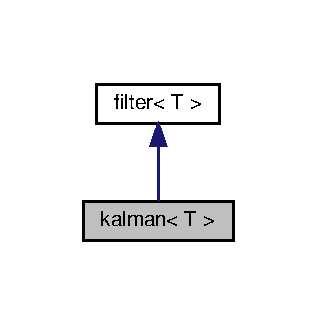
\includegraphics[width=152pt]{classkalman__inherit__graph}
\end{center}
\end{figure}


Collaboration diagram for kalman$<$ T $>$\+:\nopagebreak
\begin{figure}[H]
\begin{center}
\leavevmode
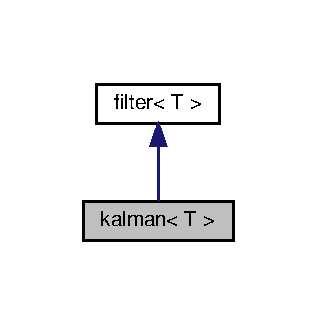
\includegraphics[width=152pt]{classkalman__coll__graph}
\end{center}
\end{figure}
\subsection*{Public Member Functions}
\begin{DoxyCompactItemize}
\item 
\hyperlink{classkalman_a8181e5861db1cf47644d9b5a02644f8b}{kalman} (const data \&A, const data \&B, const \hyperlink{classnVect}{n\+Vect}$<$ T $>$ \&i\+\_\+state, const data \&P, const data \&Q, const data \&R, const data \&I)
\begin{DoxyCompactList}\small\item\em Constructor. \end{DoxyCompactList}\item 
\hyperlink{classnVect}{n\+Vect}$<$ float $>$ \hyperlink{classkalman_ad3ce18dcca9e21b8b2cbcf25915327ac}{operator()} (const \hyperlink{classnVect}{n\+Vect}$<$ T $>$ \&measured, const float signal)
\begin{DoxyCompactList}\small\item\em () operator \end{DoxyCompactList}\item 
virtual \hyperlink{classnVect}{n\+Vect}$<$ float $>$ \hyperlink{classkalman_ae3c0c97ba8c3eb2eba0134a3adf701ed}{operator()} (\hyperlink{classnVect}{n\+Vect}$<$ T $>$ \&measured)
\begin{DoxyCompactList}\small\item\em () operator \end{DoxyCompactList}\end{DoxyCompactItemize}


\subsection{Detailed Description}
\subsubsection*{template$<$typename T$>$\newline
class kalman$<$ T $>$}

kalman class. 

This class is a derived filter class that acts as a kalman filter to filter a noisy signal from a state given a linear model. 

\subsection{Constructor \& Destructor Documentation}
\mbox{\Hypertarget{classkalman_a8181e5861db1cf47644d9b5a02644f8b}\label{classkalman_a8181e5861db1cf47644d9b5a02644f8b}} 
\index{kalman@{kalman}!kalman@{kalman}}
\index{kalman@{kalman}!kalman@{kalman}}
\subsubsection{\texorpdfstring{kalman()}{kalman()}}
{\footnotesize\ttfamily template$<$typename T $>$ \\
\hyperlink{classkalman}{kalman}$<$ T $>$\+::\hyperlink{classkalman}{kalman} (\begin{DoxyParamCaption}\item[{const data \&}]{A,  }\item[{const data \&}]{B,  }\item[{const \hyperlink{classnVect}{n\+Vect}$<$ T $>$ \&}]{i\+\_\+state,  }\item[{const data \&}]{P,  }\item[{const data \&}]{Q,  }\item[{const data \&}]{R,  }\item[{const data \&}]{I }\end{DoxyParamCaption})}



Constructor. 

Description\+: Parameterized constructor for the kalman derived filter class that allows the user to specify all constants and initial member variables for the calculations. 
\begin{DoxyParams}{Parameters}
{\em A} & is the constant state transition matrix. \\
\hline
{\em B} & is the constant input transition matrix. \\
\hline
{\em i\+\_\+state} & is the initial state of the modeled system. \\
\hline
{\em P} & is the initial state of the covariance matrix. \\
\hline
{\em Q} & is the constant process error matrix. \\
\hline
{\em R} & is the constant measurement uncertainty matrix. \\
\hline
{\em I} & is the constant identity matrix in the correct dimensions of the system. \\
\hline
\end{DoxyParams}
\begin{DoxyPostcond}{Postcondition}
A kalman filter is initialized with all the values it needs to operate. 
\end{DoxyPostcond}


\subsection{Member Function Documentation}
\mbox{\Hypertarget{classkalman_ad3ce18dcca9e21b8b2cbcf25915327ac}\label{classkalman_ad3ce18dcca9e21b8b2cbcf25915327ac}} 
\index{kalman@{kalman}!operator()@{operator()}}
\index{operator()@{operator()}!kalman@{kalman}}
\subsubsection{\texorpdfstring{operator()()}{operator()()}\hspace{0.1cm}{\footnotesize\ttfamily [1/2]}}
{\footnotesize\ttfamily template$<$typename T $>$ \\
\hyperlink{classnVect}{n\+Vect}$<$ float $>$ \hyperlink{classkalman}{kalman}$<$ T $>$\+::operator() (\begin{DoxyParamCaption}\item[{const \hyperlink{classnVect}{n\+Vect}$<$ T $>$ \&}]{measured,  }\item[{const float}]{signal }\end{DoxyParamCaption})}



() operator 

Description\+: () operator overload for the kalman derived filer that steps the simulation forward by one time step and calculates the neccessary updates for different variables. 
\begin{DoxyParams}{Parameters}
{\em measured} & is the current measured state of the system. \\
\hline
{\em signal} & is the current \hyperlink{classPID}{P\+ID} signal that was sent to the lander model. \\
\hline
\end{DoxyParams}
\begin{DoxyReturn}{Returns}
Returns a \hyperlink{classnVect}{n\+Vect$<$float$>$} that represents the filtered system. 
\end{DoxyReturn}
\begin{DoxyPrecond}{Precondition}
$\ast$, +, -\/, and = operators must be defined for type T. 
\end{DoxyPrecond}
\begin{DoxyPostcond}{Postcondition}
The filtered state is returned and the kalman filter is updated by one time step. 
\end{DoxyPostcond}
\mbox{\Hypertarget{classkalman_ae3c0c97ba8c3eb2eba0134a3adf701ed}\label{classkalman_ae3c0c97ba8c3eb2eba0134a3adf701ed}} 
\index{kalman@{kalman}!operator()@{operator()}}
\index{operator()@{operator()}!kalman@{kalman}}
\subsubsection{\texorpdfstring{operator()()}{operator()()}\hspace{0.1cm}{\footnotesize\ttfamily [2/2]}}
{\footnotesize\ttfamily template$<$typename T $>$ \\
\hyperlink{classnVect}{n\+Vect}$<$ float $>$ \hyperlink{classkalman}{kalman}$<$ T $>$\+::operator() (\begin{DoxyParamCaption}\item[{\hyperlink{classnVect}{n\+Vect}$<$ T $>$ \&}]{measured }\end{DoxyParamCaption})\hspace{0.3cm}{\ttfamily [virtual]}}



() operator 

Description\+: () operator overload that matches the virtual function defined in the filter class. This does not do anything. 
\begin{DoxyParams}{Parameters}
{\em measured} & is the current state of the system. \\
\hline
\end{DoxyParams}
\begin{DoxyReturn}{Returns}
Returns a \hyperlink{classnVect}{n\+Vect$<$float$>$} that is the same as the input. 
\end{DoxyReturn}
\begin{DoxyPostcond}{Postcondition}
Does nothing. 
\end{DoxyPostcond}


Implements \hyperlink{classfilter_ac8ec0fb4a10d10ee5e3133259610e0d2}{filter$<$ T $>$}.



The documentation for this class was generated from the following files\+:\begin{DoxyCompactItemize}
\item 
\hyperlink{kalman_8h}{kalman.\+h}\item 
kalman.\+hpp\end{DoxyCompactItemize}

\hypertarget{classlander}{}\section{lander Class Reference}
\label{classlander}\index{lander@{lander}}


lander class.  




{\ttfamily \#include $<$lander.\+h$>$}

\subsection*{Public Member Functions}
\begin{DoxyCompactItemize}
\item 
\hyperlink{classlander_ad90447438348cd18fc11a1e5c535bcc7}{lander} ()
\begin{DoxyCompactList}\small\item\em Constuctor. \end{DoxyCompactList}\item 
\hyperlink{classlander_afcc7deebd2ae6ce4391d6a29194ee42f}{lander} (const float step\+\_\+size, const std\+::initializer\+\_\+list$<$ float $>$ \&i\+\_\+state, const float set\+\_\+point)
\begin{DoxyCompactList}\small\item\em Constructor. \end{DoxyCompactList}\item 
\hyperlink{classlander_ab73cd2ea79597ebde27baf217c507f58}{lander} (const \hyperlink{classlander}{lander} \&rhs)
\begin{DoxyCompactList}\small\item\em Copy constructor Description\+: Copy constructor for the lander class that initializes a new lander object with the same values as another. \end{DoxyCompactList}\item 
\hyperlink{classlander}{lander} \& \hyperlink{classlander_af3b77c442d0872e00520a66f771cc477}{operator=} (const \hyperlink{classlander}{lander} \&rhs)
\begin{DoxyCompactList}\small\item\em = operator \end{DoxyCompactList}\item 
\hyperlink{classlander_abadffd59954f62978cee21bc59e22cfa}{$\sim$lander} ()
\begin{DoxyCompactList}\small\item\em Destructor. \end{DoxyCompactList}\item 
const float \hyperlink{classlander_a47e887be0b3b8bb2f48f6913b2917ecf}{get\+Signal} () const
\begin{DoxyCompactList}\small\item\em Signal accessor. \end{DoxyCompactList}\item 
\hyperlink{classnVect}{n\+Vect}$<$ float $>$ \hyperlink{classlander_a2fe992a7fb65bbcc59c9ce929c9a6069}{operator()} (const \hyperlink{classnVect}{n\+Vect}$<$ float $>$ \&input)
\begin{DoxyCompactList}\small\item\em () operator \end{DoxyCompactList}\end{DoxyCompactItemize}
\subsection*{Friends}
\begin{DoxyCompactItemize}
\item 
std\+::ostream \& \hyperlink{classlander_ab6f8c74d299fffd0364da0d38b9a8509}{operator$<$$<$} (std\+::ostream \&out, const \hyperlink{classlander}{lander} \&rhs)
\begin{DoxyCompactList}\small\item\em $<$$<$ operator \end{DoxyCompactList}\end{DoxyCompactItemize}


\subsection{Detailed Description}
lander class. 

This class acts acts as a model for the lander simulation that steps with a discrete time step to simulate a lander using a \hyperlink{classPID}{P\+ID} controller to correct a signal received about the landers angle measurements. 

\subsection{Constructor \& Destructor Documentation}
\mbox{\Hypertarget{classlander_ad90447438348cd18fc11a1e5c535bcc7}\label{classlander_ad90447438348cd18fc11a1e5c535bcc7}} 
\index{lander@{lander}!lander@{lander}}
\index{lander@{lander}!lander@{lander}}
\subsubsection{\texorpdfstring{lander()}{lander()}\hspace{0.1cm}{\footnotesize\ttfamily [1/3]}}
{\footnotesize\ttfamily lander\+::lander (\begin{DoxyParamCaption}{ }\end{DoxyParamCaption})}



Constuctor. 

Description\+: Default constructor for the lander class that initializes the float variables with a default value but doesn\textquotesingle{}t provide either a m\+\_\+state or m\+\_\+controller variable. \begin{DoxyPostcond}{Postcondition}
A lander class is initialized with default values for all its member variables. 
\end{DoxyPostcond}
\mbox{\Hypertarget{classlander_afcc7deebd2ae6ce4391d6a29194ee42f}\label{classlander_afcc7deebd2ae6ce4391d6a29194ee42f}} 
\index{lander@{lander}!lander@{lander}}
\index{lander@{lander}!lander@{lander}}
\subsubsection{\texorpdfstring{lander()}{lander()}\hspace{0.1cm}{\footnotesize\ttfamily [2/3]}}
{\footnotesize\ttfamily lander\+::lander (\begin{DoxyParamCaption}\item[{const float}]{step\+\_\+size,  }\item[{const std\+::initializer\+\_\+list$<$ float $>$ \&}]{i\+\_\+state,  }\item[{const float}]{set\+\_\+point }\end{DoxyParamCaption})}



Constructor. 

Description\+: Parameterized constructor for the lander class that takes a user defined step size, initial state, and \hyperlink{classPID}{P\+ID} controller to set up the lander class. 
\begin{DoxyParams}{Parameters}
{\em step\+\_\+size} & is the time step for the lander class model. \\
\hline
{\em i\+\_\+state} & is the initial state of the system represented as a \hyperlink{classnVect}{n\+Vect$<$float$>$} object. \\
\hline
{\em set\+\_\+point} & is the target set point for the theta member of the state. \\
\hline
\end{DoxyParams}
\begin{DoxyPostcond}{Postcondition}
A lander object is initialized with the proper values to perform discrete time steps on it. 
\end{DoxyPostcond}

\begin{DoxyExceptions}{Exceptions}
{\em Throws} & a std\+::domain\+\_\+error object if the step size is $<$= 0. \\
\hline
\end{DoxyExceptions}
\mbox{\Hypertarget{classlander_ab73cd2ea79597ebde27baf217c507f58}\label{classlander_ab73cd2ea79597ebde27baf217c507f58}} 
\index{lander@{lander}!lander@{lander}}
\index{lander@{lander}!lander@{lander}}
\subsubsection{\texorpdfstring{lander()}{lander()}\hspace{0.1cm}{\footnotesize\ttfamily [3/3]}}
{\footnotesize\ttfamily lander\+::lander (\begin{DoxyParamCaption}\item[{const \hyperlink{classlander}{lander} \&}]{rhs }\end{DoxyParamCaption})}



Copy constructor Description\+: Copy constructor for the lander class that initializes a new lander object with the same values as another. 


\begin{DoxyParams}{Parameters}
{\em rhs} & is the lander object to be copied. \\
\hline
\end{DoxyParams}
\begin{DoxyPostcond}{Postcondition}
A new lander object is initialized with the same value as the object passed. 
\end{DoxyPostcond}
\mbox{\Hypertarget{classlander_abadffd59954f62978cee21bc59e22cfa}\label{classlander_abadffd59954f62978cee21bc59e22cfa}} 
\index{lander@{lander}!````~lander@{$\sim$lander}}
\index{````~lander@{$\sim$lander}!lander@{lander}}
\subsubsection{\texorpdfstring{$\sim$lander()}{~lander()}}
{\footnotesize\ttfamily lander\+::$\sim$lander (\begin{DoxyParamCaption}{ }\end{DoxyParamCaption})}



Destructor. 

Description\+: Desctructor for the lander class that safely deallocates the memory of the lander object. \begin{DoxyPostcond}{Postcondition}
The lander objects reserved memory is safely deallocated. 
\end{DoxyPostcond}


\subsection{Member Function Documentation}
\mbox{\Hypertarget{classlander_a47e887be0b3b8bb2f48f6913b2917ecf}\label{classlander_a47e887be0b3b8bb2f48f6913b2917ecf}} 
\index{lander@{lander}!get\+Signal@{get\+Signal}}
\index{get\+Signal@{get\+Signal}!lander@{lander}}
\subsubsection{\texorpdfstring{get\+Signal()}{getSignal()}}
{\footnotesize\ttfamily const float lander\+::get\+Signal (\begin{DoxyParamCaption}{ }\end{DoxyParamCaption}) const}



Signal accessor. 

Description\+: Accessor for the m\+\_\+signal member variable to be output to the user. \begin{DoxyReturn}{Returns}
Returns a const float that represents the signal returned to the system from the \hyperlink{classPID}{P\+ID} controller. 
\end{DoxyReturn}
\mbox{\Hypertarget{classlander_a2fe992a7fb65bbcc59c9ce929c9a6069}\label{classlander_a2fe992a7fb65bbcc59c9ce929c9a6069}} 
\index{lander@{lander}!operator()@{operator()}}
\index{operator()@{operator()}!lander@{lander}}
\subsubsection{\texorpdfstring{operator()()}{operator()()}}
{\footnotesize\ttfamily \hyperlink{classnVect}{n\+Vect}$<$ float $>$ lander\+::operator() (\begin{DoxyParamCaption}\item[{const \hyperlink{classnVect}{n\+Vect}$<$ float $>$ \&}]{input }\end{DoxyParamCaption})}



() operator 

Description\+: () operator overload for the lander class that steps the model forward one time step. 
\begin{DoxyParams}{Parameters}
{\em input} & is the current state of the system. This allows the user to add noise and/or filter the system in between time steps. \\
\hline
\end{DoxyParams}
\begin{DoxyReturn}{Returns}
Returns a \hyperlink{classnVect}{n\+Vect$<$float$>$} to represent the updated system. 
\end{DoxyReturn}
\begin{DoxyPostcond}{Postcondition}
The model is stepped forward by one time step and the proper member variables are updated with the current values. 
\end{DoxyPostcond}
\mbox{\Hypertarget{classlander_af3b77c442d0872e00520a66f771cc477}\label{classlander_af3b77c442d0872e00520a66f771cc477}} 
\index{lander@{lander}!operator=@{operator=}}
\index{operator=@{operator=}!lander@{lander}}
\subsubsection{\texorpdfstring{operator=()}{operator=()}}
{\footnotesize\ttfamily \hyperlink{classlander}{lander} \& lander\+::operator= (\begin{DoxyParamCaption}\item[{const \hyperlink{classlander}{lander} \&}]{rhs }\end{DoxyParamCaption})}



= operator 

Description\+: = operator for the lander class that sets a lander object\textquotesingle{}s values equal to another lander. 
\begin{DoxyParams}{Parameters}
{\em rhs} & is the lander object to be copied. \\
\hline
\end{DoxyParams}
\begin{DoxyPostcond}{Postcondition}
The calling object\textquotesingle{}s variables are set equal to the object passed. 
\end{DoxyPostcond}


\subsection{Friends And Related Function Documentation}
\mbox{\Hypertarget{classlander_ab6f8c74d299fffd0364da0d38b9a8509}\label{classlander_ab6f8c74d299fffd0364da0d38b9a8509}} 
\index{lander@{lander}!operator$<$$<$@{operator$<$$<$}}
\index{operator$<$$<$@{operator$<$$<$}!lander@{lander}}
\subsubsection{\texorpdfstring{operator$<$$<$}{operator<<}}
{\footnotesize\ttfamily std\+::ostream\& operator$<$$<$ (\begin{DoxyParamCaption}\item[{std\+::ostream \&}]{out,  }\item[{const \hyperlink{classlander}{lander} \&}]{rhs }\end{DoxyParamCaption})\hspace{0.3cm}{\ttfamily [friend]}}



$<$$<$ operator 

Description\+: $<$$<$ operator overload for the lander class that allows the user to print the state information in a readable way. 
\begin{DoxyParams}{Parameters}
{\em out} & is the ostream object passed to the function. \\
\hline
{\em rhs} & is the lander object to be output to the user. \\
\hline
\end{DoxyParams}
\begin{DoxyReturn}{Returns}
Returns the ostream object. 
\end{DoxyReturn}
\begin{DoxyPostcond}{Postcondition}
The lander object is output to the user. 
\end{DoxyPostcond}


The documentation for this class was generated from the following files\+:\begin{DoxyCompactItemize}
\item 
\hyperlink{lander_8h}{lander.\+h}\item 
lander.\+hpp\end{DoxyCompactItemize}

\hypertarget{classlowPass}{}\section{low\+Pass$<$ T $>$ Class Template Reference}
\label{classlowPass}\index{low\+Pass$<$ T $>$@{low\+Pass$<$ T $>$}}


\hyperlink{classlowPass}{low\+Pass} class.  




{\ttfamily \#include $<$low\+Pass.\+h$>$}



Inheritance diagram for low\+Pass$<$ T $>$\+:\nopagebreak
\begin{figure}[H]
\begin{center}
\leavevmode
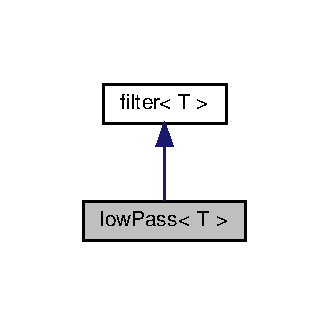
\includegraphics[width=158pt]{classlowPass__inherit__graph}
\end{center}
\end{figure}


Collaboration diagram for low\+Pass$<$ T $>$\+:\nopagebreak
\begin{figure}[H]
\begin{center}
\leavevmode
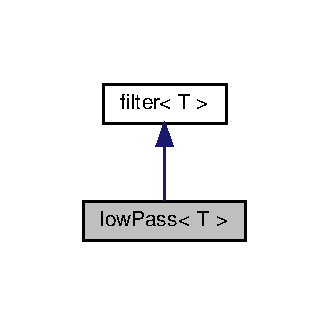
\includegraphics[width=158pt]{classlowPass__coll__graph}
\end{center}
\end{figure}
\subsection*{Public Member Functions}
\begin{DoxyCompactItemize}
\item 
\hyperlink{classlowPass_a50525f73036e6c40d03be1becbfa0068}{low\+Pass} (const float step\+Size, const float f, const \hyperlink{classnVect}{n\+Vect}$<$ T $>$ i\+\_\+state)
\begin{DoxyCompactList}\small\item\em Constructor. \end{DoxyCompactList}\item 
virtual \hyperlink{classnVect}{n\+Vect}$<$ T $>$ \hyperlink{classlowPass_a4d4458814fd69f87c5622227f6527468}{operator()} (\hyperlink{classnVect}{n\+Vect}$<$ T $>$ \&state)
\begin{DoxyCompactList}\small\item\em () operator \end{DoxyCompactList}\end{DoxyCompactItemize}


\subsection{Detailed Description}
\subsubsection*{template$<$typename T$>$\newline
class low\+Pass$<$ T $>$}

\hyperlink{classlowPass}{low\+Pass} class. 

This class acts as a \hyperlink{classlowPass}{low\+Pass} filter derived from the filter base class. 

\subsection{Constructor \& Destructor Documentation}
\mbox{\Hypertarget{classlowPass_a50525f73036e6c40d03be1becbfa0068}\label{classlowPass_a50525f73036e6c40d03be1becbfa0068}} 
\index{low\+Pass@{low\+Pass}!low\+Pass@{low\+Pass}}
\index{low\+Pass@{low\+Pass}!low\+Pass@{low\+Pass}}
\subsubsection{\texorpdfstring{low\+Pass()}{lowPass()}}
{\footnotesize\ttfamily template$<$typename T $>$ \\
\hyperlink{classlowPass}{low\+Pass}$<$ T $>$\+::\hyperlink{classlowPass}{low\+Pass} (\begin{DoxyParamCaption}\item[{const float}]{step\+Size,  }\item[{const float}]{f,  }\item[{const \hyperlink{classnVect}{n\+Vect}$<$ T $>$}]{i\+\_\+state }\end{DoxyParamCaption})}



Constructor. 

Description\+: Parameterized constructor for the \hyperlink{classlowPass}{low\+Pass} derived filter class. This constructor uses the step\+Size and f parameters to perform the more accurate calculation of alpha for the \hyperlink{classlowPass}{low\+Pass} filter method. 
\begin{DoxyParams}{Parameters}
{\em step\+Size} & is the change in time for each increment of the \hyperlink{classlowPass}{low\+Pass} filter iteration. \\
\hline
{\em f} & is the frequency for each increment of the \hyperlink{classlowPass}{low\+Pass} filter iteration. \\
\hline
{\em i\+\_\+state} & is the initial state of the system. This assumes that the state can always be represented as a vector. \\
\hline
\end{DoxyParams}
\begin{DoxyPostcond}{Postcondition}
Initializes a \hyperlink{classlowPass}{low\+Pass} filter with an alpha value and initial state that filters a noisy signal for a given state. 
\end{DoxyPostcond}


\subsection{Member Function Documentation}
\mbox{\Hypertarget{classlowPass_a4d4458814fd69f87c5622227f6527468}\label{classlowPass_a4d4458814fd69f87c5622227f6527468}} 
\index{low\+Pass@{low\+Pass}!operator()@{operator()}}
\index{operator()@{operator()}!low\+Pass@{low\+Pass}}
\subsubsection{\texorpdfstring{operator()()}{operator()()}}
{\footnotesize\ttfamily template$<$typename T $>$ \\
\hyperlink{classnVect}{n\+Vect}$<$ T $>$ \hyperlink{classlowPass}{low\+Pass}$<$ T $>$\+::operator() (\begin{DoxyParamCaption}\item[{\hyperlink{classnVect}{n\+Vect}$<$ T $>$ \&}]{state }\end{DoxyParamCaption})\hspace{0.3cm}{\ttfamily [virtual]}}



() operator 

Description\+: () operator overload for the \hyperlink{classlowPass}{low\+Pass} derived filter that takes a new state and weights that against the previous states to create a weighted average of the weighted average. 
\begin{DoxyParams}{Parameters}
{\em state} & is the current state of the system to be weighted against the current stored state m\+\_\+prev\+\_\+state. \\
\hline
\end{DoxyParams}
\begin{DoxyReturn}{Returns}
Returns the new weighted current state. 
\end{DoxyReturn}
\begin{DoxyPrecond}{Precondition}
$\ast$ and + operators must be defined for type T. 
\end{DoxyPrecond}
\begin{DoxyPostcond}{Postcondition}
The previous state is updated with the proper weights of the previous and current states. 
\end{DoxyPostcond}


Implements \hyperlink{classfilter_ac8ec0fb4a10d10ee5e3133259610e0d2}{filter$<$ T $>$}.



The documentation for this class was generated from the following files\+:\begin{DoxyCompactItemize}
\item 
\hyperlink{lowPass_8h}{low\+Pass.\+h}\item 
low\+Pass.\+hpp\end{DoxyCompactItemize}

\hypertarget{classnTrix}{}\section{n\+Trix$<$ T $>$ Class Template Reference}
\label{classnTrix}\index{n\+Trix$<$ T $>$@{n\+Trix$<$ T $>$}}


\hyperlink{classnTrix}{n\+Trix} class.  




{\ttfamily \#include $<$n\+Trix.\+h$>$}

\subsection*{Public Member Functions}
\begin{DoxyCompactItemize}
\item 
\hyperlink{classnTrix_a1f99b7fa79bb2f28ffd014591c55d3a1}{n\+Trix} ()
\begin{DoxyCompactList}\small\item\em Default Constructor. \end{DoxyCompactList}\item 
\hyperlink{classnTrix_ad7dd393c0056a77c9ebeb551112e2f7c}{n\+Trix} (const std\+::initializer\+\_\+list$<$ std\+::initializer\+\_\+list$<$ T $>$$>$ \&grid)
\begin{DoxyCompactList}\small\item\em Constructor. \end{DoxyCompactList}\item 
\hyperlink{classnTrix_ac0b8db0c386024c87d57b8c0e3a31c65}{n\+Trix} (const short num\+\_\+rows, const short num\+\_\+cols)
\begin{DoxyCompactList}\small\item\em Constructor. \end{DoxyCompactList}\item 
\hyperlink{classnTrix_a702b976039784b4b6d699c929f835270}{n\+Trix} (const \hyperlink{classnVect}{n\+Vect}$<$ T $>$ \&rhs)
\begin{DoxyCompactList}\small\item\em Vector Constructor. \end{DoxyCompactList}\item 
\hyperlink{classnTrix_a490ebc8fb7a94e577b33e05b16daafec}{n\+Trix} (const \hyperlink{classnTrix}{n\+Trix}$<$ T $>$ \&rhs)
\begin{DoxyCompactList}\small\item\em Copy Constructor. \end{DoxyCompactList}\item 
\hyperlink{classnTrix}{n\+Trix}$<$ T $>$ \& \hyperlink{classnTrix_a9003760685902f4e9f5759f826906641}{operator=} (const \hyperlink{classnTrix}{n\+Trix}$<$ T $>$ \&rhs)
\begin{DoxyCompactList}\small\item\em = operator \end{DoxyCompactList}\item 
\hyperlink{classnTrix_a9f0136573e29a5196bee15e35983e1f8}{$\sim$n\+Trix} ()
\begin{DoxyCompactList}\small\item\em Destructor. \end{DoxyCompactList}\item 
short \hyperlink{classnTrix_a1b837cfb3182d38894e86a252cbc5ce1}{rows} () const
\begin{DoxyCompactList}\small\item\em Row accessor. \end{DoxyCompactList}\item 
short \hyperlink{classnTrix_ad0995ceefe1049d39280e139db121358}{cols} () const
\begin{DoxyCompactList}\small\item\em Column accessor. \end{DoxyCompactList}\item 
const T \& \hyperlink{classnTrix_a0b575b4c1a79ba858e081ab8cc53ef20}{operator()} (const int row\+\_\+index, const int col\+\_\+index) const
\begin{DoxyCompactList}\small\item\em Index accessor. \end{DoxyCompactList}\item 
float \hyperlink{classnTrix_afd682a4691502bcdd530c0580b13b05e}{one\+\_\+norm} () const
\begin{DoxyCompactList}\small\item\em One norm calculator. \end{DoxyCompactList}\item 
float \hyperlink{classnTrix_aa21e2d162693c9f031fcd69936d27485}{infinity\+\_\+norm} () const
\begin{DoxyCompactList}\small\item\em Infinity norm calculator. \end{DoxyCompactList}\item 
float \hyperlink{classnTrix_a072250efd8048da611e8b42eda8458ad}{frobenius} () const
\begin{DoxyCompactList}\small\item\em frobenius norm \end{DoxyCompactList}\item 
T \& \hyperlink{classnTrix_af53f20ac6f018adc7e850a6ed34fb5fe}{operator()} (const int row\+\_\+index, const int col\+\_\+index)
\begin{DoxyCompactList}\small\item\em Index accessor. \end{DoxyCompactList}\item 
\hyperlink{classnTrix}{n\+Trix}$<$ T $>$ \hyperlink{classnTrix_aacf51597babef6c97ba7101066f84157}{operator+} (const \hyperlink{classnTrix}{n\+Trix}$<$ T $>$ \&rhs) const
\begin{DoxyCompactList}\small\item\em 
\begin{DoxyItemize}
\item operator 
\end{DoxyItemize}\end{DoxyCompactList}\item 
\hyperlink{classnTrix}{n\+Trix}$<$ T $>$ \hyperlink{classnTrix_af43db03d2939e1ccb8f218f3d55543e8}{operator-\/} (const \hyperlink{classnTrix}{n\+Trix}$<$ T $>$ \&rhs) const
\begin{DoxyCompactList}\small\item\em Binary -\/ operator. \end{DoxyCompactList}\item 
\hyperlink{classnTrix}{n\+Trix}$<$ T $>$ \hyperlink{classnTrix_a23acc805ad0f69ca5f8195327ebdc3f2}{operator-\/} () const
\begin{DoxyCompactList}\small\item\em Unary -\/ operator. \end{DoxyCompactList}\item 
\hyperlink{classnTrix}{n\+Trix}$<$ T $>$ \hyperlink{classnTrix_ad04ab9579b2941f7be4b0402085fd40f}{operator$\ast$} (const \hyperlink{classnTrix}{n\+Trix}$<$ T $>$ \&rhs) const
\begin{DoxyCompactList}\small\item\em 
\begin{DoxyItemize}
\item operator 
\end{DoxyItemize}\end{DoxyCompactList}\item 
\hyperlink{classnVect}{n\+Vect}$<$ T $>$ \hyperlink{classnTrix_a6e3a9b2026a59a6822b060abf6d97425}{operator$\ast$} (const \hyperlink{classnVect}{n\+Vect}$<$ T $>$ \&rhs) const
\begin{DoxyCompactList}\small\item\em 
\begin{DoxyItemize}
\item operator 
\end{DoxyItemize}\end{DoxyCompactList}\item 
void \hyperlink{classnTrix_a709740bd4cf9fe868849e6e3de8189f2}{clear} ()
\begin{DoxyCompactList}\small\item\em Clear function. \end{DoxyCompactList}\item 
\hyperlink{classnTrix}{n\+Trix}$<$ float $>$ \hyperlink{classnTrix_af96c6e8b9eceb4e8a173969db7fdf938}{invert} () const
\begin{DoxyCompactList}\small\item\em invert function \end{DoxyCompactList}\item 
\hyperlink{classnTrix}{n\+Trix}$<$ T $>$ \hyperlink{classnTrix_ab0ac2336544d0957fd8b4ee2d99179b9}{transpose} () const
\begin{DoxyCompactList}\small\item\em Transpose function. \end{DoxyCompactList}\end{DoxyCompactItemize}
\subsection*{Friends}
\begin{DoxyCompactItemize}
\item 
{\footnotesize template$<$typename U $>$ }\\std\+::ostream \& \hyperlink{classnTrix_a3c1676bdc29761ac82a51c65977ca769}{operator$<$$<$} (std\+::ostream \&out, const \hyperlink{classnTrix}{n\+Trix}$<$ U $>$ \&rhs)
\begin{DoxyCompactList}\small\item\em $<$$<$ operator \end{DoxyCompactList}\item 
{\footnotesize template$<$typename U $>$ }\\std\+::istream \& \hyperlink{classnTrix_a08d2697db68d298a32870ce310782313}{operator$>$$>$} (std\+::istream \&in, \hyperlink{classnTrix}{n\+Trix}$<$ U $>$ \&rhs)
\begin{DoxyCompactList}\small\item\em \begin{quote}
\begin{quote}
operator\end{quote}
\end{quote}
\end{DoxyCompactList}\end{DoxyCompactItemize}


\subsection{Detailed Description}
\subsubsection*{template$<$typename T$>$\newline
class n\+Trix$<$ T $>$}

\hyperlink{classnTrix}{n\+Trix} class. 

This class uses an array of pointers to simulate a 2D array for matrix implementation 

\subsection{Constructor \& Destructor Documentation}
\mbox{\Hypertarget{classnTrix_a1f99b7fa79bb2f28ffd014591c55d3a1}\label{classnTrix_a1f99b7fa79bb2f28ffd014591c55d3a1}} 
\index{n\+Trix@{n\+Trix}!n\+Trix@{n\+Trix}}
\index{n\+Trix@{n\+Trix}!n\+Trix@{n\+Trix}}
\subsubsection{\texorpdfstring{n\+Trix()}{nTrix()}\hspace{0.1cm}{\footnotesize\ttfamily [1/5]}}
{\footnotesize\ttfamily template$<$typename T $>$ \\
\hyperlink{classnTrix}{n\+Trix}$<$ T $>$\+::\hyperlink{classnTrix}{n\+Trix} (\begin{DoxyParamCaption}{ }\end{DoxyParamCaption})}



Default Constructor. 

Description\+: Creates a default 2x2 matrix. \begin{DoxyPostcond}{Postcondition}
A 2x2 matrix is initialized with no values stored. 
\end{DoxyPostcond}
\mbox{\Hypertarget{classnTrix_ad7dd393c0056a77c9ebeb551112e2f7c}\label{classnTrix_ad7dd393c0056a77c9ebeb551112e2f7c}} 
\index{n\+Trix@{n\+Trix}!n\+Trix@{n\+Trix}}
\index{n\+Trix@{n\+Trix}!n\+Trix@{n\+Trix}}
\subsubsection{\texorpdfstring{n\+Trix()}{nTrix()}\hspace{0.1cm}{\footnotesize\ttfamily [2/5]}}
{\footnotesize\ttfamily template$<$typename T $>$ \\
\hyperlink{classnTrix}{n\+Trix}$<$ T $>$\+::\hyperlink{classnTrix}{n\+Trix} (\begin{DoxyParamCaption}\item[{const std\+::initializer\+\_\+list$<$ std\+::initializer\+\_\+list$<$ T $>$$>$ \&}]{grid }\end{DoxyParamCaption})}



Constructor. 

Description\+: A constructor that accepts a std\+::initializer\+\_\+list of std\+::initializer\+\_\+list$<$\+T$>$ to fill a matrix with the values specified. 
\begin{DoxyParams}{Parameters}
{\em grid} & is a list of lists that store the values to be input into the matrix. \\
\hline
\end{DoxyParams}
\begin{DoxyPrecond}{Precondition}
= operator must be defined for type T. 
\end{DoxyPrecond}
\begin{DoxyPostcond}{Postcondition}
A matrix is initialized with the dimensions and values of the list of lists passed. 
\end{DoxyPostcond}

\begin{DoxyExceptions}{Exceptions}
{\em Throws} & a std\+::domain\+\_\+error object if one of the lists is not the same length as the others. \\
\hline
\end{DoxyExceptions}
\mbox{\Hypertarget{classnTrix_ac0b8db0c386024c87d57b8c0e3a31c65}\label{classnTrix_ac0b8db0c386024c87d57b8c0e3a31c65}} 
\index{n\+Trix@{n\+Trix}!n\+Trix@{n\+Trix}}
\index{n\+Trix@{n\+Trix}!n\+Trix@{n\+Trix}}
\subsubsection{\texorpdfstring{n\+Trix()}{nTrix()}\hspace{0.1cm}{\footnotesize\ttfamily [3/5]}}
{\footnotesize\ttfamily template$<$typename T $>$ \\
\hyperlink{classnTrix}{n\+Trix}$<$ T $>$\+::\hyperlink{classnTrix}{n\+Trix} (\begin{DoxyParamCaption}\item[{const short}]{num\+\_\+rows,  }\item[{const short}]{num\+\_\+cols }\end{DoxyParamCaption})}



Constructor. 

Description\+: Constructs a matrix of size num\+\_\+rows x num\+\_\+cols with no values stored. 
\begin{DoxyParams}{Parameters}
{\em num\+\_\+rows} & is the number of rows for the matrix. \\
\hline
{\em num\+\_\+cols} & is the number of columns for the matrix. \\
\hline
\end{DoxyParams}
\begin{DoxyPostcond}{Postcondition}
A r x c matrix is initialized with no values stored. 
\end{DoxyPostcond}

\begin{DoxyExceptions}{Exceptions}
{\em Throws} & a std\+::domain\+\_\+error object if either of the dimensions are negative. \\
\hline
\end{DoxyExceptions}
\mbox{\Hypertarget{classnTrix_a702b976039784b4b6d699c929f835270}\label{classnTrix_a702b976039784b4b6d699c929f835270}} 
\index{n\+Trix@{n\+Trix}!n\+Trix@{n\+Trix}}
\index{n\+Trix@{n\+Trix}!n\+Trix@{n\+Trix}}
\subsubsection{\texorpdfstring{n\+Trix()}{nTrix()}\hspace{0.1cm}{\footnotesize\ttfamily [4/5]}}
{\footnotesize\ttfamily template$<$typename T $>$ \\
\hyperlink{classnTrix}{n\+Trix}$<$ T $>$\+::\hyperlink{classnTrix}{n\+Trix} (\begin{DoxyParamCaption}\item[{const \hyperlink{classnVect}{n\+Vect}$<$ T $>$ \&}]{rhs }\end{DoxyParamCaption})}



Vector Constructor. 

Description\+: Allows a matrix to be constructed based on a \hyperlink{classnVect}{n\+Vect} vector. The matrix is a column matrix. 
\begin{DoxyParams}{Parameters}
{\em rhs} & is the \hyperlink{classnVect}{n\+Vect} to be copied. \\
\hline
\end{DoxyParams}
\begin{DoxyPrecond}{Precondition}
= operator needs to be defined for type T. 
\end{DoxyPrecond}
\begin{DoxyPostcond}{Postcondition}
A column matrix is constructed with the same values in the \hyperlink{classnVect}{n\+Vect}. 
\end{DoxyPostcond}
\mbox{\Hypertarget{classnTrix_a490ebc8fb7a94e577b33e05b16daafec}\label{classnTrix_a490ebc8fb7a94e577b33e05b16daafec}} 
\index{n\+Trix@{n\+Trix}!n\+Trix@{n\+Trix}}
\index{n\+Trix@{n\+Trix}!n\+Trix@{n\+Trix}}
\subsubsection{\texorpdfstring{n\+Trix()}{nTrix()}\hspace{0.1cm}{\footnotesize\ttfamily [5/5]}}
{\footnotesize\ttfamily template$<$typename T $>$ \\
\hyperlink{classnTrix}{n\+Trix}$<$ T $>$\+::\hyperlink{classnTrix}{n\+Trix} (\begin{DoxyParamCaption}\item[{const \hyperlink{classnTrix}{n\+Trix}$<$ T $>$ \&}]{rhs }\end{DoxyParamCaption})}



Copy Constructor. 

Description\+: Copy constructor that initializes a new matrix with the same values as the matrix passed. 
\begin{DoxyParams}{Parameters}
{\em rhs} & is the matrix to be copied. \\
\hline
\end{DoxyParams}
\begin{DoxyPrecond}{Precondition}
= operator needs to be defined for type T. 
\end{DoxyPrecond}
\begin{DoxyPostcond}{Postcondition}
A new matrix is initialized with the same values as the one passed. 
\end{DoxyPostcond}
\mbox{\Hypertarget{classnTrix_a9f0136573e29a5196bee15e35983e1f8}\label{classnTrix_a9f0136573e29a5196bee15e35983e1f8}} 
\index{n\+Trix@{n\+Trix}!````~n\+Trix@{$\sim$n\+Trix}}
\index{````~n\+Trix@{$\sim$n\+Trix}!n\+Trix@{n\+Trix}}
\subsubsection{\texorpdfstring{$\sim$n\+Trix()}{~nTrix()}}
{\footnotesize\ttfamily template$<$typename T $>$ \\
\hyperlink{classnTrix}{n\+Trix}$<$ T $>$\+::$\sim$\hyperlink{classnTrix}{n\+Trix} (\begin{DoxyParamCaption}{ }\end{DoxyParamCaption})}



Destructor. 

Description\+: Properly destructs a \hyperlink{classnTrix}{n\+Trix} object to avoid memory leaks. \begin{DoxyPostcond}{Postcondition}
The calling object is safely destructed. 
\end{DoxyPostcond}


\subsection{Member Function Documentation}
\mbox{\Hypertarget{classnTrix_a709740bd4cf9fe868849e6e3de8189f2}\label{classnTrix_a709740bd4cf9fe868849e6e3de8189f2}} 
\index{n\+Trix@{n\+Trix}!clear@{clear}}
\index{clear@{clear}!n\+Trix@{n\+Trix}}
\subsubsection{\texorpdfstring{clear()}{clear()}}
{\footnotesize\ttfamily template$<$typename T $>$ \\
void \hyperlink{classnTrix}{n\+Trix}$<$ T $>$\+::clear (\begin{DoxyParamCaption}{ }\end{DoxyParamCaption})}



Clear function. 

Description\+: Allows the user to clear a \hyperlink{classnTrix}{n\+Trix} object. \begin{DoxyPostcond}{Postcondition}
All of the calling object\textquotesingle{}s data is erased and the size is set to 0x0. 
\end{DoxyPostcond}
\mbox{\Hypertarget{classnTrix_ad0995ceefe1049d39280e139db121358}\label{classnTrix_ad0995ceefe1049d39280e139db121358}} 
\index{n\+Trix@{n\+Trix}!cols@{cols}}
\index{cols@{cols}!n\+Trix@{n\+Trix}}
\subsubsection{\texorpdfstring{cols()}{cols()}}
{\footnotesize\ttfamily template$<$typename T $>$ \\
short \hyperlink{classnTrix}{n\+Trix}$<$ T $>$\+::cols (\begin{DoxyParamCaption}{ }\end{DoxyParamCaption}) const}



Column accessor. 

Description\+: Returns the number of columns in a matrix. \begin{DoxyReturn}{Returns}
The number of columns in a matrix. 
\end{DoxyReturn}
\mbox{\Hypertarget{classnTrix_a072250efd8048da611e8b42eda8458ad}\label{classnTrix_a072250efd8048da611e8b42eda8458ad}} 
\index{n\+Trix@{n\+Trix}!frobenius@{frobenius}}
\index{frobenius@{frobenius}!n\+Trix@{n\+Trix}}
\subsubsection{\texorpdfstring{frobenius()}{frobenius()}}
{\footnotesize\ttfamily template$<$typename T $>$ \\
float \hyperlink{classnTrix}{n\+Trix}$<$ T $>$\+::frobenius (\begin{DoxyParamCaption}{ }\end{DoxyParamCaption}) const}



frobenius norm 

Description\+: Two norm calculator for matrices. \begin{DoxyReturn}{Returns}
returns the frobenius norm of the matrix as a float. 
\end{DoxyReturn}
\begin{DoxyPrecond}{Precondition}
$\ast$ operator must be defined for type T. 
\end{DoxyPrecond}
\mbox{\Hypertarget{classnTrix_aa21e2d162693c9f031fcd69936d27485}\label{classnTrix_aa21e2d162693c9f031fcd69936d27485}} 
\index{n\+Trix@{n\+Trix}!infinity\+\_\+norm@{infinity\+\_\+norm}}
\index{infinity\+\_\+norm@{infinity\+\_\+norm}!n\+Trix@{n\+Trix}}
\subsubsection{\texorpdfstring{infinity\+\_\+norm()}{infinity\_norm()}}
{\footnotesize\ttfamily template$<$typename T $>$ \\
float \hyperlink{classnTrix}{n\+Trix}$<$ T $>$\+::infinity\+\_\+norm (\begin{DoxyParamCaption}{ }\end{DoxyParamCaption}) const}



Infinity norm calculator. 

Description\+: Calculates the infinity-\/norm or the maximum row sum of a matrix. \begin{DoxyReturn}{Returns}
Returns a float that represents the maximum row sum. 
\end{DoxyReturn}
\begin{DoxyPrecond}{Precondition}
std\+::abs() needs to be defined for type T. 

+= operator needs to be defined for type T. 
\end{DoxyPrecond}
\mbox{\Hypertarget{classnTrix_af96c6e8b9eceb4e8a173969db7fdf938}\label{classnTrix_af96c6e8b9eceb4e8a173969db7fdf938}} 
\index{n\+Trix@{n\+Trix}!invert@{invert}}
\index{invert@{invert}!n\+Trix@{n\+Trix}}
\subsubsection{\texorpdfstring{invert()}{invert()}}
{\footnotesize\ttfamily template$<$typename T $>$ \\
\hyperlink{classnTrix}{n\+Trix}$<$ float $>$ \hyperlink{classnTrix}{n\+Trix}$<$ T $>$\+::invert (\begin{DoxyParamCaption}{ }\end{DoxyParamCaption}) const}



invert function 

Description\+: Inverts the calling object using the Newton-\/\+Schultz iterative method for inverting a matrix. \begin{DoxyReturn}{Returns}
Returns a n\+Trix$<$float$>$ that represents the inverted calling object. 
\end{DoxyReturn}
\begin{DoxyPostcond}{Postcondition}
Calls the \hyperlink{nTrix_8h_acb6ffe9fd3e8aa373a570884247ac35b}{r\+\_\+invert()} function to recursively iterate the matrix. 
\end{DoxyPostcond}

\begin{DoxyExceptions}{Exceptions}
{\em Throws} & a std\+::range\+\_\+error object if the object is not a square matrix. \\
\hline
\end{DoxyExceptions}
\mbox{\Hypertarget{classnTrix_afd682a4691502bcdd530c0580b13b05e}\label{classnTrix_afd682a4691502bcdd530c0580b13b05e}} 
\index{n\+Trix@{n\+Trix}!one\+\_\+norm@{one\+\_\+norm}}
\index{one\+\_\+norm@{one\+\_\+norm}!n\+Trix@{n\+Trix}}
\subsubsection{\texorpdfstring{one\+\_\+norm()}{one\_norm()}}
{\footnotesize\ttfamily template$<$typename T $>$ \\
float \hyperlink{classnTrix}{n\+Trix}$<$ T $>$\+::one\+\_\+norm (\begin{DoxyParamCaption}{ }\end{DoxyParamCaption}) const}



One norm calculator. 

Description\+: Calculates the one-\/norm or the maximum column sum of a matrix. \begin{DoxyReturn}{Returns}
Returns a float that represents the maximum column sum. 
\end{DoxyReturn}
\begin{DoxyPrecond}{Precondition}
std\+::abs() needs to be defined for type T. 

+= operator needs to be defined for type T. 
\end{DoxyPrecond}
\mbox{\Hypertarget{classnTrix_a0b575b4c1a79ba858e081ab8cc53ef20}\label{classnTrix_a0b575b4c1a79ba858e081ab8cc53ef20}} 
\index{n\+Trix@{n\+Trix}!operator()@{operator()}}
\index{operator()@{operator()}!n\+Trix@{n\+Trix}}
\subsubsection{\texorpdfstring{operator()()}{operator()()}\hspace{0.1cm}{\footnotesize\ttfamily [1/2]}}
{\footnotesize\ttfamily template$<$typename T $>$ \\
const T \& \hyperlink{classnTrix}{n\+Trix}$<$ T $>$\+::operator() (\begin{DoxyParamCaption}\item[{const int}]{row\+\_\+index,  }\item[{const int}]{col\+\_\+index }\end{DoxyParamCaption}) const}



Index accessor. 

Description\+: Allows the user to view the i,j-\/th element in the matrix. 
\begin{DoxyParams}{Parameters}
{\em row\+\_\+index} & is the row to view. \\
\hline
{\em col\+\_\+index} & is the column member of the row to view. \\
\hline
\end{DoxyParams}
\begin{DoxyReturn}{Returns}
Returns a const reference to the T object at that index in the matrix. 
\end{DoxyReturn}

\begin{DoxyExceptions}{Exceptions}
{\em Throws} & a std\+::domain\+\_\+error object if either of the indexes are less than zero or greater than their respective domains that they are attempting to access. \\
\hline
\end{DoxyExceptions}
\mbox{\Hypertarget{classnTrix_af53f20ac6f018adc7e850a6ed34fb5fe}\label{classnTrix_af53f20ac6f018adc7e850a6ed34fb5fe}} 
\index{n\+Trix@{n\+Trix}!operator()@{operator()}}
\index{operator()@{operator()}!n\+Trix@{n\+Trix}}
\subsubsection{\texorpdfstring{operator()()}{operator()()}\hspace{0.1cm}{\footnotesize\ttfamily [2/2]}}
{\footnotesize\ttfamily template$<$typename T $>$ \\
T \& \hyperlink{classnTrix}{n\+Trix}$<$ T $>$\+::operator() (\begin{DoxyParamCaption}\item[{const int}]{row\+\_\+index,  }\item[{const int}]{col\+\_\+index }\end{DoxyParamCaption})}



Index accessor. 

Description\+: Allows the user to access the i,j-\/th element in the matrix. 
\begin{DoxyParams}{Parameters}
{\em row\+\_\+index} & is the row to view. \\
\hline
{\em col\+\_\+index} & is the column member of the row to view. \\
\hline
\end{DoxyParams}
\begin{DoxyReturn}{Returns}
Returns a reference to the T object at that index in the matrix. 
\end{DoxyReturn}

\begin{DoxyExceptions}{Exceptions}
{\em Throws} & a std\+::domain\+\_\+error object if either of the indexes are less than zero or greater than their respective domains that they are attempting to access. \\
\hline
\end{DoxyExceptions}
\mbox{\Hypertarget{classnTrix_ad04ab9579b2941f7be4b0402085fd40f}\label{classnTrix_ad04ab9579b2941f7be4b0402085fd40f}} 
\index{n\+Trix@{n\+Trix}!operator$\ast$@{operator$\ast$}}
\index{operator$\ast$@{operator$\ast$}!n\+Trix@{n\+Trix}}
\subsubsection{\texorpdfstring{operator$\ast$()}{operator*()}\hspace{0.1cm}{\footnotesize\ttfamily [1/2]}}
{\footnotesize\ttfamily template$<$typename T $>$ \\
\hyperlink{classnTrix}{n\+Trix}$<$ T $>$ \hyperlink{classnTrix}{n\+Trix}$<$ T $>$\+::operator$\ast$ (\begin{DoxyParamCaption}\item[{const \hyperlink{classnTrix}{n\+Trix}$<$ T $>$ \&}]{rhs }\end{DoxyParamCaption}) const}




\begin{DoxyItemize}
\item operator 
\end{DoxyItemize}

Description\+: $\ast$ operator overload for the \hyperlink{classnTrix}{n\+Trix} class that allows the user to multiply two \hyperlink{classnTrix}{n\+Trix} objects of the same type. 
\begin{DoxyParams}{Parameters}
{\em rhs} & is the \hyperlink{classnTrix}{n\+Trix} to be multiplied with the calling object. \\
\hline
\end{DoxyParams}
\begin{DoxyReturn}{Returns}
Returns a new \hyperlink{classnTrix}{n\+Trix} that is the product of the calling object and the object passed. 
\end{DoxyReturn}
\begin{DoxyPrecond}{Precondition}
$\ast$ operator must be defined for type T. 
\end{DoxyPrecond}

\begin{DoxyExceptions}{Exceptions}
{\em Throws} & a std\+::invalid\+\_\+argument object if the two matrices are not the correct dimensions for matrix multiplication to occur. \\
\hline
\end{DoxyExceptions}
\mbox{\Hypertarget{classnTrix_a6e3a9b2026a59a6822b060abf6d97425}\label{classnTrix_a6e3a9b2026a59a6822b060abf6d97425}} 
\index{n\+Trix@{n\+Trix}!operator$\ast$@{operator$\ast$}}
\index{operator$\ast$@{operator$\ast$}!n\+Trix@{n\+Trix}}
\subsubsection{\texorpdfstring{operator$\ast$()}{operator*()}\hspace{0.1cm}{\footnotesize\ttfamily [2/2]}}
{\footnotesize\ttfamily template$<$typename T $>$ \\
\hyperlink{classnVect}{n\+Vect}$<$ T $>$ \hyperlink{classnTrix}{n\+Trix}$<$ T $>$\+::operator$\ast$ (\begin{DoxyParamCaption}\item[{const \hyperlink{classnVect}{n\+Vect}$<$ T $>$ \&}]{rhs }\end{DoxyParamCaption}) const}




\begin{DoxyItemize}
\item operator 
\end{DoxyItemize}

Description\+: $\ast$ operator overload for the \hyperlink{classnTrix}{n\+Trix} class that allows the user to multiply a matrix with a vector. 
\begin{DoxyParams}{Parameters}
{\em rhs} & is a \hyperlink{classnVect}{n\+Vect} object to be multiplied to a \hyperlink{classnTrix}{n\+Trix}. \\
\hline
\end{DoxyParams}
\begin{DoxyReturn}{Returns}
Returns a n\+Vect$<$\+T$>$ object with the values having matrix multiplicaion applied. 
\end{DoxyReturn}
\begin{DoxyPrecond}{Precondition}
$\ast$ operator must be defined for type T. 
\end{DoxyPrecond}

\begin{DoxyExceptions}{Exceptions}
{\em Throws} & a std\+::invalid\+\_\+argument object if the vector and matrix are not the correct dimensions for multiplication to occur. \\
\hline
\end{DoxyExceptions}
\mbox{\Hypertarget{classnTrix_aacf51597babef6c97ba7101066f84157}\label{classnTrix_aacf51597babef6c97ba7101066f84157}} 
\index{n\+Trix@{n\+Trix}!operator+@{operator+}}
\index{operator+@{operator+}!n\+Trix@{n\+Trix}}
\subsubsection{\texorpdfstring{operator+()}{operator+()}}
{\footnotesize\ttfamily template$<$typename T $>$ \\
\hyperlink{classnTrix}{n\+Trix}$<$ T $>$ \hyperlink{classnTrix}{n\+Trix}$<$ T $>$\+::operator+ (\begin{DoxyParamCaption}\item[{const \hyperlink{classnTrix}{n\+Trix}$<$ T $>$ \&}]{rhs }\end{DoxyParamCaption}) const}




\begin{DoxyItemize}
\item operator 
\end{DoxyItemize}

Description\+: + operator overload for the \hyperlink{classnTrix}{n\+Trix} class that allows for the addition of two \hyperlink{classnTrix}{n\+Trix} objects. 
\begin{DoxyParams}{Parameters}
{\em rhs} & is the \hyperlink{classnTrix}{n\+Trix} to be added to the calling object. \\
\hline
\end{DoxyParams}
\begin{DoxyReturn}{Returns}
Returns a new matrix that is the sum of the calling object and the object passed. 
\end{DoxyReturn}
\begin{DoxyPrecond}{Precondition}
+= operator needs to be defined for type T. 
\end{DoxyPrecond}

\begin{DoxyExceptions}{Exceptions}
{\em Throws} & a std\+::invalid\+\_\+argument object if the matrices are not the same size. \\
\hline
\end{DoxyExceptions}
\mbox{\Hypertarget{classnTrix_af43db03d2939e1ccb8f218f3d55543e8}\label{classnTrix_af43db03d2939e1ccb8f218f3d55543e8}} 
\index{n\+Trix@{n\+Trix}!operator-\/@{operator-\/}}
\index{operator-\/@{operator-\/}!n\+Trix@{n\+Trix}}
\subsubsection{\texorpdfstring{operator-\/()}{operator-()}\hspace{0.1cm}{\footnotesize\ttfamily [1/2]}}
{\footnotesize\ttfamily template$<$typename T $>$ \\
\hyperlink{classnTrix}{n\+Trix}$<$ T $>$ \hyperlink{classnTrix}{n\+Trix}$<$ T $>$\+::operator-\/ (\begin{DoxyParamCaption}\item[{const \hyperlink{classnTrix}{n\+Trix}$<$ T $>$ \&}]{rhs }\end{DoxyParamCaption}) const}



Binary -\/ operator. 

Description\+: -\/ operator overload for the \hyperlink{classnTrix}{n\+Trix} class that allows for the subtraction of two \hyperlink{classnTrix}{n\+Trix} objects. 
\begin{DoxyParams}{Parameters}
{\em rhs} & is the \hyperlink{classnTrix}{n\+Trix} to be subtracted from the calling object. \\
\hline
\end{DoxyParams}
\begin{DoxyReturn}{Returns}
Returns a new matrix that is the difference of the calling object and the object passed. 
\end{DoxyReturn}
\begin{DoxyPrecond}{Precondition}
$\ast$ operator must be defined for type T. 

+= operator must be defined for type T. 
\end{DoxyPrecond}

\begin{DoxyExceptions}{Exceptions}
{\em Throws} & a std\+::invalid\+\_\+argument object if the matrices are not the same size. \\
\hline
\end{DoxyExceptions}
\mbox{\Hypertarget{classnTrix_a23acc805ad0f69ca5f8195327ebdc3f2}\label{classnTrix_a23acc805ad0f69ca5f8195327ebdc3f2}} 
\index{n\+Trix@{n\+Trix}!operator-\/@{operator-\/}}
\index{operator-\/@{operator-\/}!n\+Trix@{n\+Trix}}
\subsubsection{\texorpdfstring{operator-\/()}{operator-()}\hspace{0.1cm}{\footnotesize\ttfamily [2/2]}}
{\footnotesize\ttfamily template$<$typename T $>$ \\
\hyperlink{classnTrix}{n\+Trix}$<$ T $>$ \hyperlink{classnTrix}{n\+Trix}$<$ T $>$\+::operator-\/ (\begin{DoxyParamCaption}{ }\end{DoxyParamCaption}) const}



Unary -\/ operator. 

Description\+: -\/ operator overload for the \hyperlink{classnTrix}{n\+Trix} class that negates every element in the matrix. \begin{DoxyReturn}{Returns}
Returns a new \hyperlink{classnTrix}{n\+Trix} with all values from the calling object negated. 
\end{DoxyReturn}
\begin{DoxyPrecond}{Precondition}
$\ast$ operator must be defined for type T. 
\end{DoxyPrecond}
\mbox{\Hypertarget{classnTrix_a9003760685902f4e9f5759f826906641}\label{classnTrix_a9003760685902f4e9f5759f826906641}} 
\index{n\+Trix@{n\+Trix}!operator=@{operator=}}
\index{operator=@{operator=}!n\+Trix@{n\+Trix}}
\subsubsection{\texorpdfstring{operator=()}{operator=()}}
{\footnotesize\ttfamily template$<$typename T $>$ \\
\hyperlink{classnTrix}{n\+Trix}$<$ T $>$ \& \hyperlink{classnTrix}{n\+Trix}$<$ T $>$\+::operator= (\begin{DoxyParamCaption}\item[{const \hyperlink{classnTrix}{n\+Trix}$<$ T $>$ \&}]{rhs }\end{DoxyParamCaption})}



= operator 

Description\+: = operator for the \hyperlink{classnTrix}{n\+Trix} class that sets the calling object equal to the object passed. 
\begin{DoxyParams}{Parameters}
{\em rhs} & is the matrix to be copied. \\
\hline
\end{DoxyParams}
\begin{DoxyReturn}{Returns}
Returns $\ast$this with the copied values. 
\end{DoxyReturn}
\begin{DoxyPrecond}{Precondition}
= operator needs to be defined for type T. 
\end{DoxyPrecond}
\begin{DoxyPostcond}{Postcondition}
The calling object is set equal to the object passed. 
\end{DoxyPostcond}
\mbox{\Hypertarget{classnTrix_a1b837cfb3182d38894e86a252cbc5ce1}\label{classnTrix_a1b837cfb3182d38894e86a252cbc5ce1}} 
\index{n\+Trix@{n\+Trix}!rows@{rows}}
\index{rows@{rows}!n\+Trix@{n\+Trix}}
\subsubsection{\texorpdfstring{rows()}{rows()}}
{\footnotesize\ttfamily template$<$typename T $>$ \\
short \hyperlink{classnTrix}{n\+Trix}$<$ T $>$\+::rows (\begin{DoxyParamCaption}{ }\end{DoxyParamCaption}) const}



Row accessor. 

Description\+: Returns the number of rows in a matrix. \begin{DoxyReturn}{Returns}
The number of rows in a matrix. 
\end{DoxyReturn}
\mbox{\Hypertarget{classnTrix_ab0ac2336544d0957fd8b4ee2d99179b9}\label{classnTrix_ab0ac2336544d0957fd8b4ee2d99179b9}} 
\index{n\+Trix@{n\+Trix}!transpose@{transpose}}
\index{transpose@{transpose}!n\+Trix@{n\+Trix}}
\subsubsection{\texorpdfstring{transpose()}{transpose()}}
{\footnotesize\ttfamily template$<$typename T $>$ \\
\hyperlink{classnTrix}{n\+Trix}$<$ T $>$ \hyperlink{classnTrix}{n\+Trix}$<$ T $>$\+::transpose (\begin{DoxyParamCaption}{ }\end{DoxyParamCaption}) const}



Transpose function. 

Description\+: Calculates the transpose of a matrix. \begin{DoxyReturn}{Returns}
Returns a new n\+Trix$<$\+T$>$ that is the transpose of the calling object. 
\end{DoxyReturn}
\begin{DoxyPrecond}{Precondition}
= operator must be defined for type T. 
\end{DoxyPrecond}


\subsection{Friends And Related Function Documentation}
\mbox{\Hypertarget{classnTrix_a3c1676bdc29761ac82a51c65977ca769}\label{classnTrix_a3c1676bdc29761ac82a51c65977ca769}} 
\index{n\+Trix@{n\+Trix}!operator$<$$<$@{operator$<$$<$}}
\index{operator$<$$<$@{operator$<$$<$}!n\+Trix@{n\+Trix}}
\subsubsection{\texorpdfstring{operator$<$$<$}{operator<<}}
{\footnotesize\ttfamily template$<$typename T$>$ \\
template$<$typename U $>$ \\
std\+::ostream\& operator$<$$<$ (\begin{DoxyParamCaption}\item[{std\+::ostream \&}]{out,  }\item[{const \hyperlink{classnTrix}{n\+Trix}$<$ U $>$ \&}]{rhs }\end{DoxyParamCaption})\hspace{0.3cm}{\ttfamily [friend]}}



$<$$<$ operator 

Description\+: $<$$<$ operator overloaded to pretty print the \hyperlink{classnTrix}{n\+Trix} object. 
\begin{DoxyParams}{Parameters}
{\em out} & is the ostream object passed to the function. \\
\hline
{\em rhs} & is the n\+Trix$<$\+T$>$ object to be output. \\
\hline
\end{DoxyParams}
\begin{DoxyReturn}{Returns}
Returns the ostream. 
\end{DoxyReturn}
\begin{DoxyPrecond}{Precondition}
$<$$<$ operator must be defined for type T. 
\end{DoxyPrecond}
\begin{DoxyPostcond}{Postcondition}
Outputs the matrix to the user. 
\end{DoxyPostcond}
\mbox{\Hypertarget{classnTrix_a08d2697db68d298a32870ce310782313}\label{classnTrix_a08d2697db68d298a32870ce310782313}} 
\index{n\+Trix@{n\+Trix}!operator$>$$>$@{operator$>$$>$}}
\index{operator$>$$>$@{operator$>$$>$}!n\+Trix@{n\+Trix}}
\subsubsection{\texorpdfstring{operator$>$$>$}{operator>>}}
{\footnotesize\ttfamily template$<$typename T$>$ \\
template$<$typename U $>$ \\
std\+::istream\& operator$>$$>$ (\begin{DoxyParamCaption}\item[{std\+::istream \&}]{in,  }\item[{\hyperlink{classnTrix}{n\+Trix}$<$ U $>$ \&}]{rhs }\end{DoxyParamCaption})\hspace{0.3cm}{\ttfamily [friend]}}



\begin{quote}
\begin{quote}
operator\end{quote}
\end{quote}


Description\+: $>$$>$ operator overloaded to extract a matrix object from the istream. The inputted matrix overloads any previously stored data in the \hyperlink{classnTrix}{n\+Trix} object. 
\begin{DoxyParams}{Parameters}
{\em in} & is the istream object passed to the function. \\
\hline
{\em rhs} & is the n\+Trix$<$\+T$>$ object to store the input. \\
\hline
\end{DoxyParams}
\begin{DoxyReturn}{Returns}
Returns the istream. 
\end{DoxyReturn}
\begin{DoxyPrecond}{Precondition}
$>$$>$ operator must be defined for type T. 
\end{DoxyPrecond}
\begin{DoxyPostcond}{Postcondition}
Stores the input in the object passed. 
\end{DoxyPostcond}

\begin{DoxyExceptions}{Exceptions}
{\em Throws} & a std\+::range\+\_\+error object if the user inputs an incorrect number of items for a column. \\
\hline
\end{DoxyExceptions}


The documentation for this class was generated from the following files\+:\begin{DoxyCompactItemize}
\item 
\hyperlink{nTrix_8h}{n\+Trix.\+h}\item 
n\+Trix.\+hpp\end{DoxyCompactItemize}

\hypertarget{classnVect}{}\section{n\+Vect$<$ T $>$ Class Template Reference}
\label{classnVect}\index{n\+Vect$<$ T $>$@{n\+Vect$<$ T $>$}}


\hyperlink{classnVect}{n\+Vect} class.  




{\ttfamily \#include $<$n\+Vect.\+h$>$}

\subsection*{Classes}
\begin{DoxyCompactItemize}
\item 
class \hyperlink{classnVect_1_1iterator}{iterator}
\begin{DoxyCompactList}\small\item\em iterator class. \end{DoxyCompactList}\end{DoxyCompactItemize}
\subsection*{Public Member Functions}
\begin{DoxyCompactItemize}
\item 
\hyperlink{classnVect_abb7dc7935aeb2e8f6811b1f0e4c0fb40}{n\+Vect} ()
\begin{DoxyCompactList}\small\item\em Default constructor. \end{DoxyCompactList}\item 
\hyperlink{classnVect_a1b72b4f2c2ca8fadc844936ed6c82d5b}{n\+Vect} (const int \hyperlink{classnVect_a5cf871204b41c5cd97055b3c4ee9607c}{size})
\begin{DoxyCompactList}\small\item\em Constructor. \end{DoxyCompactList}\item 
\hyperlink{classnVect_a8b77a6ebdc28746d61eebb7d8bbc0691}{n\+Vect} (const std\+::initializer\+\_\+list$<$ T $>$ \&list)
\begin{DoxyCompactList}\small\item\em constructor \end{DoxyCompactList}\item 
\hyperlink{classnVect_ad47ea98ac300eeaa3aab9322bfe20e76}{n\+Vect} (const \hyperlink{classnVect}{n\+Vect}$<$ T $>$ \&cpy\+\_\+vec)
\begin{DoxyCompactList}\small\item\em copy constructor \end{DoxyCompactList}\item 
\hyperlink{classnVect}{n\+Vect}$<$ T $>$ \& \hyperlink{classnVect_a47cd80bc62dec71439736d6f0218d57e}{operator=} (const \hyperlink{classnVect}{n\+Vect}$<$ T $>$ \&cpy\+\_\+vec)
\begin{DoxyCompactList}\small\item\em = operator \end{DoxyCompactList}\item 
\hyperlink{classnVect_a7d537e5be0ce55f3ea40e43c54cdb9a7}{$\sim$n\+Vect} ()
\begin{DoxyCompactList}\small\item\em destructor \end{DoxyCompactList}\item 
void \hyperlink{classnVect_aac4b9c9287c14f0957f46eec00f17e62}{push\+\_\+back} (const T \&item)
\begin{DoxyCompactList}\small\item\em Adds an element to the back of the vector. \end{DoxyCompactList}\item 
void \hyperlink{classnVect_a5d998eac73178b38c0e24a6aa29eacbb}{resize} (const int new\+\_\+size)
\begin{DoxyCompactList}\small\item\em Sets a new size for the vector. \end{DoxyCompactList}\item 
void \hyperlink{classnVect_a58dcec4cc5ea9d8d18e03fb1671bee2b}{resize} (const int new\+\_\+size, const T \&filler)
\begin{DoxyCompactList}\small\item\em Sets a new size for the vector and fills it. \end{DoxyCompactList}\item 
void \hyperlink{classnVect_ad83c522fff7a545b02d20dbf2e99a4e7}{clear} ()
\begin{DoxyCompactList}\small\item\em clears the object \end{DoxyCompactList}\item 
T \& \hyperlink{classnVect_a3fb4c0900764f5b46c402639a1baf01f}{operator\mbox{[}$\,$\mbox{]}} (const int index)
\begin{DoxyCompactList}\small\item\em \mbox{[}\mbox{]} operator reference \end{DoxyCompactList}\item 
\hyperlink{classnVect}{n\+Vect}$<$ T $>$ \hyperlink{classnVect_a2941f0e337b1c7348e8b479539ea715c}{operator-\/} (const \hyperlink{classnVect}{n\+Vect}$<$ T $>$ \&rhs)
\begin{DoxyCompactList}\small\item\em 
\begin{DoxyItemize}
\item operator (binary) 
\end{DoxyItemize}\end{DoxyCompactList}\item 
\hyperlink{classnVect}{n\+Vect}$<$ T $>$ \hyperlink{classnVect_a24677bbe43b1a1f5d77b36e7b96bcb98}{operator-\/} ()
\begin{DoxyCompactList}\small\item\em unary minus \end{DoxyCompactList}\item 
\hyperlink{classnVect}{n\+Vect}$<$ T $>$ \hyperlink{classnVect_a35964beca3a57fad4f69ddd6be16cc91}{apply} (T func(T)) const
\begin{DoxyCompactList}\small\item\em apply function \end{DoxyCompactList}\item 
T \& \hyperlink{classnVect_a4b757cc98836654ee2929197d40d9055}{get} (const int index)
\begin{DoxyCompactList}\small\item\em get function \end{DoxyCompactList}\item 
int \hyperlink{classnVect_a5cf871204b41c5cd97055b3c4ee9607c}{size} () const
\begin{DoxyCompactList}\small\item\em size of the vector \end{DoxyCompactList}\item 
const T \& \hyperlink{classnVect_a65b439185fd34563833ede9390612f1c}{operator\mbox{[}$\,$\mbox{]}} (const int index) const
\begin{DoxyCompactList}\small\item\em \mbox{[}\mbox{]} operator const \end{DoxyCompactList}\item 
T \hyperlink{classnVect_ac5933c6480457c627ca43a8b9d1cfbaf}{operator$\ast$} (const \hyperlink{classnVect}{n\+Vect}$<$ T $>$ \&rhs) const
\begin{DoxyCompactList}\small\item\em Vector multiplication. \end{DoxyCompactList}\item 
double \hyperlink{classnVect_a32237bab9097b7b392c467a79d858d1a}{operator$^\wedge$} (const int norm) const
\begin{DoxyCompactList}\small\item\em P-\/norm calculator. \end{DoxyCompactList}\item 
\hyperlink{classnVect_1_1iterator}{iterator} \hyperlink{classnVect_a0daf09e1f15ac627815d57f777ecc417}{begin} ()
\begin{DoxyCompactList}\small\item\em starting iterator \end{DoxyCompactList}\item 
\hyperlink{classnVect_1_1iterator}{iterator} \hyperlink{classnVect_a44a13c3cb3ede92ae23298920b1d88bf}{end} ()
\begin{DoxyCompactList}\small\item\em ending iterator \end{DoxyCompactList}\end{DoxyCompactItemize}
\subsection*{Friends}
\begin{DoxyCompactItemize}
\item 
{\footnotesize template$<$typename U $>$ }\\\hyperlink{classnVect}{n\+Vect}$<$ U $>$ \hyperlink{classnVect_a3ffde125079f1f4fdfc8e99d6a714439}{operator+} (const \hyperlink{classnVect}{n\+Vect}$<$ U $>$ \&lhs, const \hyperlink{classnVect}{n\+Vect}$<$ U $>$ \&rhs)
\begin{DoxyCompactList}\small\item\em 
\begin{DoxyItemize}
\item operator 
\end{DoxyItemize}\end{DoxyCompactList}\item 
{\footnotesize template$<$typename U $>$ }\\\hyperlink{classnVect}{n\+Vect}$<$ U $>$ \hyperlink{classnVect_a64c439aa3f26ec0fea5c63a6e52a1be2}{operator$\ast$} (const \hyperlink{classnVect}{n\+Vect}$<$ U $>$ \&lhs, const U \&rhs)
\begin{DoxyCompactList}\small\item\em Scalar multiplication. \end{DoxyCompactList}\item 
{\footnotesize template$<$typename U $>$ }\\\hyperlink{classnVect}{n\+Vect}$<$ U $>$ \hyperlink{classnVect_a9673bd479b1647b3f4ed8a68b1b793a9}{operator$\ast$} (const U \&lhs, const \hyperlink{classnVect}{n\+Vect}$<$ U $>$ \&rhs)
\begin{DoxyCompactList}\small\item\em Scalar multiplication. \end{DoxyCompactList}\item 
{\footnotesize template$<$typename U $>$ }\\std\+::ostream \& \hyperlink{classnVect_a6b1efa03bac435bc6ce49d8de18ad3e5}{operator$<$$<$} (std\+::ostream \&out, const \hyperlink{classnVect}{n\+Vect}$<$ U $>$ \&rhs)
\begin{DoxyCompactList}\small\item\em $<$$<$ operator \end{DoxyCompactList}\item 
{\footnotesize template$<$typename U $>$ }\\std\+::istream \& \hyperlink{classnVect_ad614110b01ea7a7d8618a95d46186916}{operator$>$$>$} (std\+::istream \&in, const \hyperlink{classnVect}{n\+Vect}$<$ U $>$ \&rhs)
\begin{DoxyCompactList}\small\item\em \begin{quote}
\begin{quote}
operator\end{quote}
\end{quote}
\end{DoxyCompactList}\end{DoxyCompactItemize}


\subsection{Detailed Description}
\subsubsection*{template$<$typename T$>$\newline
class n\+Vect$<$ T $>$}

\hyperlink{classnVect}{n\+Vect} class. 

This class uses std\+::arrays to create a vector and dynamically allocate memory. 

\subsection{Constructor \& Destructor Documentation}
\mbox{\Hypertarget{classnVect_abb7dc7935aeb2e8f6811b1f0e4c0fb40}\label{classnVect_abb7dc7935aeb2e8f6811b1f0e4c0fb40}} 
\index{n\+Vect@{n\+Vect}!n\+Vect@{n\+Vect}}
\index{n\+Vect@{n\+Vect}!n\+Vect@{n\+Vect}}
\subsubsection{\texorpdfstring{n\+Vect()}{nVect()}\hspace{0.1cm}{\footnotesize\ttfamily [1/4]}}
{\footnotesize\ttfamily template$<$typename T $>$ \\
\hyperlink{classnVect}{n\+Vect}$<$ T $>$\+::\hyperlink{classnVect}{n\+Vect} (\begin{DoxyParamCaption}{ }\end{DoxyParamCaption})}



Default constructor. 

Description\+: Creates an empty vector of type T, sets m\+\_\+size to 0 and m\+\_\+available to 10. \begin{DoxyPostcond}{Postcondition}
A \hyperlink{classnVect}{n\+Vect} object is created with nothing stored and a maximum of 10 spaces available. 
\end{DoxyPostcond}
\mbox{\Hypertarget{classnVect_a1b72b4f2c2ca8fadc844936ed6c82d5b}\label{classnVect_a1b72b4f2c2ca8fadc844936ed6c82d5b}} 
\index{n\+Vect@{n\+Vect}!n\+Vect@{n\+Vect}}
\index{n\+Vect@{n\+Vect}!n\+Vect@{n\+Vect}}
\subsubsection{\texorpdfstring{n\+Vect()}{nVect()}\hspace{0.1cm}{\footnotesize\ttfamily [2/4]}}
{\footnotesize\ttfamily template$<$typename T $>$ \\
\hyperlink{classnVect}{n\+Vect}$<$ T $>$\+::\hyperlink{classnVect}{n\+Vect} (\begin{DoxyParamCaption}\item[{const int}]{size }\end{DoxyParamCaption})}



Constructor. 

Description\+: Takes an integer size and initializes a \hyperlink{classnVect}{n\+Vect} with that size available. It initializes the space but fills it with nothing. 
\begin{DoxyParams}{Parameters}
{\em size} & is the integer size of the vector to be created. \\
\hline
\end{DoxyParams}
\begin{DoxyPrecond}{Precondition}
The array allocated is filled with zeroes. 
\end{DoxyPrecond}
\begin{DoxyPostcond}{Postcondition}
A \hyperlink{classnVect}{n\+Vect} object is created with zeroes stored and (size) elements available. 
\end{DoxyPostcond}

\begin{DoxyExceptions}{Exceptions}
{\em throws} & a std\+::length\+\_\+error object if the size is negative. \\
\hline
\end{DoxyExceptions}
\mbox{\Hypertarget{classnVect_a8b77a6ebdc28746d61eebb7d8bbc0691}\label{classnVect_a8b77a6ebdc28746d61eebb7d8bbc0691}} 
\index{n\+Vect@{n\+Vect}!n\+Vect@{n\+Vect}}
\index{n\+Vect@{n\+Vect}!n\+Vect@{n\+Vect}}
\subsubsection{\texorpdfstring{n\+Vect()}{nVect()}\hspace{0.1cm}{\footnotesize\ttfamily [3/4]}}
{\footnotesize\ttfamily template$<$typename T$>$ \\
\hyperlink{classnVect}{n\+Vect}$<$ T $>$\+::\hyperlink{classnVect}{n\+Vect} (\begin{DoxyParamCaption}\item[{const std\+::initializer\+\_\+list$<$ T $>$ \&}]{list }\end{DoxyParamCaption})}



constructor 

Description\+: Constructs a \hyperlink{classnVect}{n\+Vect} object based off of the std\+::initializer\+\_\+list passed to it. 
\begin{DoxyParams}{Parameters}
{\em list} & is a std\+::initializer\+\_\+list that stores the elements to be stored in the \hyperlink{classnVect}{n\+Vect}. \\
\hline
\end{DoxyParams}
\begin{DoxyPostcond}{Postcondition}
A \hyperlink{classnVect}{n\+Vect} object is created with the data and size equal to the data and size of the std\+::initializer\+\_\+list. 
\end{DoxyPostcond}
\mbox{\Hypertarget{classnVect_ad47ea98ac300eeaa3aab9322bfe20e76}\label{classnVect_ad47ea98ac300eeaa3aab9322bfe20e76}} 
\index{n\+Vect@{n\+Vect}!n\+Vect@{n\+Vect}}
\index{n\+Vect@{n\+Vect}!n\+Vect@{n\+Vect}}
\subsubsection{\texorpdfstring{n\+Vect()}{nVect()}\hspace{0.1cm}{\footnotesize\ttfamily [4/4]}}
{\footnotesize\ttfamily template$<$typename T$>$ \\
\hyperlink{classnVect}{n\+Vect}$<$ T $>$\+::\hyperlink{classnVect}{n\+Vect} (\begin{DoxyParamCaption}\item[{const \hyperlink{classnVect}{n\+Vect}$<$ T $>$ \&}]{cpy\+\_\+vec }\end{DoxyParamCaption})}



copy constructor 

Description\+: Constructs a \hyperlink{classnVect}{n\+Vect} object with all member variables set equal to the \hyperlink{classnVect}{n\+Vect} passed. 
\begin{DoxyParams}{Parameters}
{\em cpy\+\_\+vec} & is a \hyperlink{classnVect}{n\+Vect} that has already been initialized with data. \\
\hline
\end{DoxyParams}
\begin{DoxyPostcond}{Postcondition}
The newly initialized \hyperlink{classnVect}{n\+Vect} is created and has all data set equal to the cpy\+\_\+vec passed. 
\end{DoxyPostcond}
\mbox{\Hypertarget{classnVect_a7d537e5be0ce55f3ea40e43c54cdb9a7}\label{classnVect_a7d537e5be0ce55f3ea40e43c54cdb9a7}} 
\index{n\+Vect@{n\+Vect}!````~n\+Vect@{$\sim$n\+Vect}}
\index{````~n\+Vect@{$\sim$n\+Vect}!n\+Vect@{n\+Vect}}
\subsubsection{\texorpdfstring{$\sim$n\+Vect()}{~nVect()}}
{\footnotesize\ttfamily template$<$typename T $>$ \\
\hyperlink{classnVect}{n\+Vect}$<$ T $>$\+::$\sim$\hyperlink{classnVect}{n\+Vect} (\begin{DoxyParamCaption}{ }\end{DoxyParamCaption})}



destructor 

Description\+: Properly deallocates memory for the \hyperlink{classnVect}{n\+Vect} class. \begin{DoxyPostcond}{Postcondition}
The calling object has its memory properly deallocated. 
\end{DoxyPostcond}


\subsection{Member Function Documentation}
\mbox{\Hypertarget{classnVect_a35964beca3a57fad4f69ddd6be16cc91}\label{classnVect_a35964beca3a57fad4f69ddd6be16cc91}} 
\index{n\+Vect@{n\+Vect}!apply@{apply}}
\index{apply@{apply}!n\+Vect@{n\+Vect}}
\subsubsection{\texorpdfstring{apply()}{apply()}}
{\footnotesize\ttfamily template$<$typename T$>$ \\
\hyperlink{classnVect}{n\+Vect}$<$ T $>$ \hyperlink{classnVect}{n\+Vect}$<$ T $>$\+::apply (\begin{DoxyParamCaption}\item[{T }]{funcT }\end{DoxyParamCaption}) const}



apply function 

Description\+: Allows the user to pass a function that takes a type T and returns a type T. apply applies the function to each container. 
\begin{DoxyParams}{Parameters}
{\em func} & is a function that takes a type T and returns a type T. \\
\hline
\end{DoxyParams}
\begin{DoxyReturn}{Returns}
Returns a new vector based off of the calling object with func applied to each container. 
\end{DoxyReturn}
\begin{DoxyPostcond}{Postcondition}
Creates a new vector that gets returned. 
\end{DoxyPostcond}
\mbox{\Hypertarget{classnVect_a0daf09e1f15ac627815d57f777ecc417}\label{classnVect_a0daf09e1f15ac627815d57f777ecc417}} 
\index{n\+Vect@{n\+Vect}!begin@{begin}}
\index{begin@{begin}!n\+Vect@{n\+Vect}}
\subsubsection{\texorpdfstring{begin()}{begin()}}
{\footnotesize\ttfamily template$<$typename T$>$ \\
\hyperlink{classnVect_1_1iterator}{iterator} \hyperlink{classnVect}{n\+Vect}$<$ T $>$\+::begin (\begin{DoxyParamCaption}{ }\end{DoxyParamCaption})\hspace{0.3cm}{\ttfamily [inline]}}



starting iterator 

Description\+: Returns an iterator pointing to the beginning of the \hyperlink{classnVect}{n\+Vect} object\textquotesingle{}s array. \begin{DoxyReturn}{Returns}
Returns a new iterator object that points to the start of the \hyperlink{classnVect}{n\+Vect} array. 
\end{DoxyReturn}
\begin{DoxyPrecond}{Precondition}
The first index in the vector that stores data needs to be m\+\_\+arr\mbox{[}0\mbox{]}. 
\end{DoxyPrecond}
\mbox{\Hypertarget{classnVect_ad83c522fff7a545b02d20dbf2e99a4e7}\label{classnVect_ad83c522fff7a545b02d20dbf2e99a4e7}} 
\index{n\+Vect@{n\+Vect}!clear@{clear}}
\index{clear@{clear}!n\+Vect@{n\+Vect}}
\subsubsection{\texorpdfstring{clear()}{clear()}}
{\footnotesize\ttfamily template$<$typename T $>$ \\
void \hyperlink{classnVect}{n\+Vect}$<$ T $>$\+::clear (\begin{DoxyParamCaption}{ }\end{DoxyParamCaption})}



clears the object 

Description\+: wipes the objects, sets m\+\_\+size and m\+\_\+available to 0 and makes m\+\_\+arr N\+U\+LL. \begin{DoxyPostcond}{Postcondition}
All data stored in the vector is deleted and all variables are set to a base state of 0/\+N\+U\+LL. 
\end{DoxyPostcond}
\mbox{\Hypertarget{classnVect_a44a13c3cb3ede92ae23298920b1d88bf}\label{classnVect_a44a13c3cb3ede92ae23298920b1d88bf}} 
\index{n\+Vect@{n\+Vect}!end@{end}}
\index{end@{end}!n\+Vect@{n\+Vect}}
\subsubsection{\texorpdfstring{end()}{end()}}
{\footnotesize\ttfamily template$<$typename T$>$ \\
\hyperlink{classnVect_1_1iterator}{iterator} \hyperlink{classnVect}{n\+Vect}$<$ T $>$\+::end (\begin{DoxyParamCaption}{ }\end{DoxyParamCaption})\hspace{0.3cm}{\ttfamily [inline]}}



ending iterator 

Description\+: Returns an iterator pointing to the ending of the \hyperlink{classnVect}{n\+Vect} object\textquotesingle{}s array. \begin{DoxyReturn}{Returns}
Returns a new iterator object that points to the end of the \hyperlink{classnVect}{n\+Vect} array. 
\end{DoxyReturn}
\mbox{\Hypertarget{classnVect_a4b757cc98836654ee2929197d40d9055}\label{classnVect_a4b757cc98836654ee2929197d40d9055}} 
\index{n\+Vect@{n\+Vect}!get@{get}}
\index{get@{get}!n\+Vect@{n\+Vect}}
\subsubsection{\texorpdfstring{get()}{get()}}
{\footnotesize\ttfamily template$<$typename T $>$ \\
T \& \hyperlink{classnVect}{n\+Vect}$<$ T $>$\+::get (\begin{DoxyParamCaption}\item[{const int}]{index }\end{DoxyParamCaption})}



get function 

Description\+: Returns a reference to the data stored in the container at position index in the array. 
\begin{DoxyParams}{Parameters}
{\em index} & is the index in the vector to be accessed. \\
\hline
\end{DoxyParams}
\begin{DoxyReturn}{Returns}
Returns a reference to the element at the index in the vector. 
\end{DoxyReturn}
\begin{DoxyPrecond}{Precondition}
0 $<$= index $<$ m\+\_\+size 
\end{DoxyPrecond}

\begin{DoxyExceptions}{Exceptions}
{\em Throws} & a std\+::domain\+\_\+error object if index is out of bounds. \\
\hline
\end{DoxyExceptions}
\mbox{\Hypertarget{classnVect_ac5933c6480457c627ca43a8b9d1cfbaf}\label{classnVect_ac5933c6480457c627ca43a8b9d1cfbaf}} 
\index{n\+Vect@{n\+Vect}!operator$\ast$@{operator$\ast$}}
\index{operator$\ast$@{operator$\ast$}!n\+Vect@{n\+Vect}}
\subsubsection{\texorpdfstring{operator$\ast$()}{operator*()}}
{\footnotesize\ttfamily template$<$typename T$>$ \\
T \hyperlink{classnVect}{n\+Vect}$<$ T $>$\+::operator$\ast$ (\begin{DoxyParamCaption}\item[{const \hyperlink{classnVect}{n\+Vect}$<$ T $>$ \&}]{rhs }\end{DoxyParamCaption}) const}



Vector multiplication. 

Description\+: Calculates the dot product of the parameter and calling object vectors and returns the scalar. 
\begin{DoxyParams}{Parameters}
{\em rhs} & is the vector to be dotted with the calling object. \\
\hline
\end{DoxyParams}
\begin{DoxyReturn}{Returns}
Returns a scalar representing the dot product of the vectors. 
\end{DoxyReturn}
\begin{DoxyPrecond}{Precondition}
$\ast$ and += operators need to be defined for type T. 
\end{DoxyPrecond}
\mbox{\Hypertarget{classnVect_a2941f0e337b1c7348e8b479539ea715c}\label{classnVect_a2941f0e337b1c7348e8b479539ea715c}} 
\index{n\+Vect@{n\+Vect}!operator-\/@{operator-\/}}
\index{operator-\/@{operator-\/}!n\+Vect@{n\+Vect}}
\subsubsection{\texorpdfstring{operator-\/()}{operator-()}\hspace{0.1cm}{\footnotesize\ttfamily [1/2]}}
{\footnotesize\ttfamily template$<$typename T$>$ \\
\hyperlink{classnVect}{n\+Vect}$<$ T $>$ \hyperlink{classnVect}{n\+Vect}$<$ T $>$\+::operator-\/ (\begin{DoxyParamCaption}\item[{const \hyperlink{classnVect}{n\+Vect}$<$ T $>$ \&}]{rhs }\end{DoxyParamCaption})}




\begin{DoxyItemize}
\item operator (binary) 
\end{DoxyItemize}

Description\+: Used to subtract one vector from another. Allows for vectors of different (or similar) sizes to be added through vector subtraction. 
\begin{DoxyParams}{Parameters}
{\em rhs} & is the vector to be subtracted from the calling object. \\
\hline
\end{DoxyParams}
\begin{DoxyReturn}{Returns}
Returns a newly created vector where each container now holds the difference of the two vectors passed at that index. 
\end{DoxyReturn}
\begin{DoxyPrecond}{Precondition}
-\/= operator needs to be defined for type T. 
\end{DoxyPrecond}
\begin{DoxyPostcond}{Postcondition}
Creates a new vector that gets returned. 
\end{DoxyPostcond}
\mbox{\Hypertarget{classnVect_a24677bbe43b1a1f5d77b36e7b96bcb98}\label{classnVect_a24677bbe43b1a1f5d77b36e7b96bcb98}} 
\index{n\+Vect@{n\+Vect}!operator-\/@{operator-\/}}
\index{operator-\/@{operator-\/}!n\+Vect@{n\+Vect}}
\subsubsection{\texorpdfstring{operator-\/()}{operator-()}\hspace{0.1cm}{\footnotesize\ttfamily [2/2]}}
{\footnotesize\ttfamily template$<$typename T$>$ \\
\hyperlink{classnVect}{n\+Vect}$<$ T $>$ \hyperlink{classnVect}{n\+Vect}$<$ T $>$\+::operator-\/ (\begin{DoxyParamCaption}{ }\end{DoxyParamCaption})}



unary minus 

Description\+: Negates a calling vector. \begin{DoxyReturn}{Returns}
Returns a newly created vector that is equal to the negative of the calling object. 
\end{DoxyReturn}
\begin{DoxyPrecond}{Precondition}
$\ast$= operator needs to be defined for type T. 
\end{DoxyPrecond}
\begin{DoxyPostcond}{Postcondition}
Creates a new vector that gets returned. 
\end{DoxyPostcond}
\mbox{\Hypertarget{classnVect_a47cd80bc62dec71439736d6f0218d57e}\label{classnVect_a47cd80bc62dec71439736d6f0218d57e}} 
\index{n\+Vect@{n\+Vect}!operator=@{operator=}}
\index{operator=@{operator=}!n\+Vect@{n\+Vect}}
\subsubsection{\texorpdfstring{operator=()}{operator=()}}
{\footnotesize\ttfamily template$<$typename T$>$ \\
\hyperlink{classnVect}{n\+Vect}$<$ T $>$ \& \hyperlink{classnVect}{n\+Vect}$<$ T $>$\+::operator= (\begin{DoxyParamCaption}\item[{const \hyperlink{classnVect}{n\+Vect}$<$ T $>$ \&}]{cpy\+\_\+vec }\end{DoxyParamCaption})}



= operator 

Description\+: Sets the calling object equal to the parameter. 
\begin{DoxyParams}{Parameters}
{\em cpy\+\_\+vec} & is a \hyperlink{classnVect}{n\+Vect} that has already been initialized with data. \\
\hline
\end{DoxyParams}
\begin{DoxyReturn}{Returns}
returns a \hyperlink{classnVect}{n\+Vect} through $\ast$this. 
\end{DoxyReturn}
\begin{DoxyPrecond}{Precondition}
operator = needs to be defined for type T. 
\end{DoxyPrecond}
\begin{DoxyPostcond}{Postcondition}
The calling object is set equal to the parameter. 
\end{DoxyPostcond}
\mbox{\Hypertarget{classnVect_a3fb4c0900764f5b46c402639a1baf01f}\label{classnVect_a3fb4c0900764f5b46c402639a1baf01f}} 
\index{n\+Vect@{n\+Vect}!operator\mbox{[}\mbox{]}@{operator[]}}
\index{operator\mbox{[}\mbox{]}@{operator[]}!n\+Vect@{n\+Vect}}
\subsubsection{\texorpdfstring{operator[]()}{operator[]()}\hspace{0.1cm}{\footnotesize\ttfamily [1/2]}}
{\footnotesize\ttfamily template$<$typename T $>$ \\
T \& \hyperlink{classnVect}{n\+Vect}$<$ T $>$\+::operator\mbox{[}$\,$\mbox{]} (\begin{DoxyParamCaption}\item[{const int}]{index }\end{DoxyParamCaption})}



\mbox{[}\mbox{]} operator reference 

Description\+: Allows the user to access an index in the array. 
\begin{DoxyParams}{Parameters}
{\em index} & is the space in the vector to be accessed. \\
\hline
\end{DoxyParams}
\begin{DoxyReturn}{Returns}
Returns the value at the index in the vector. 
\end{DoxyReturn}
\begin{DoxyPrecond}{Precondition}
0 $<$= index $<$ m\+\_\+size 
\end{DoxyPrecond}

\begin{DoxyExceptions}{Exceptions}
{\em Throws} & a std\+::domain\+\_\+error object is the index is out of bounds. \\
\hline
\end{DoxyExceptions}
\mbox{\Hypertarget{classnVect_a65b439185fd34563833ede9390612f1c}\label{classnVect_a65b439185fd34563833ede9390612f1c}} 
\index{n\+Vect@{n\+Vect}!operator\mbox{[}\mbox{]}@{operator[]}}
\index{operator\mbox{[}\mbox{]}@{operator[]}!n\+Vect@{n\+Vect}}
\subsubsection{\texorpdfstring{operator[]()}{operator[]()}\hspace{0.1cm}{\footnotesize\ttfamily [2/2]}}
{\footnotesize\ttfamily template$<$typename T $>$ \\
const T \& \hyperlink{classnVect}{n\+Vect}$<$ T $>$\+::operator\mbox{[}$\,$\mbox{]} (\begin{DoxyParamCaption}\item[{const int}]{index }\end{DoxyParamCaption}) const}



\mbox{[}\mbox{]} operator const 

Description\+: Allows for safe accessing of the data at the certain index in the vector. 
\begin{DoxyParams}{Parameters}
{\em index} & is the index in the vector to be accessed. \\
\hline
\end{DoxyParams}
\begin{DoxyReturn}{Returns}
Returns a const reference to the data stored at that index. 
\end{DoxyReturn}
\begin{DoxyPrecond}{Precondition}
0 $<$= index $<$ m\+\_\+size 
\end{DoxyPrecond}

\begin{DoxyExceptions}{Exceptions}
{\em Throws} & a std\+::domain\+\_\+error if index is out of bounds. \\
\hline
\end{DoxyExceptions}
\mbox{\Hypertarget{classnVect_a32237bab9097b7b392c467a79d858d1a}\label{classnVect_a32237bab9097b7b392c467a79d858d1a}} 
\index{n\+Vect@{n\+Vect}!operator$^\wedge$@{operator$^\wedge$}}
\index{operator$^\wedge$@{operator$^\wedge$}!n\+Vect@{n\+Vect}}
\subsubsection{\texorpdfstring{operator$^\wedge$()}{operator^()}}
{\footnotesize\ttfamily template$<$typename T $>$ \\
double \hyperlink{classnVect}{n\+Vect}$<$ T $>$\+::operator$^\wedge$ (\begin{DoxyParamCaption}\item[{const int}]{norm }\end{DoxyParamCaption}) const}



P-\/norm calculator. 

Description\+: Calculates the p-\/norm for a given \hyperlink{classnVect}{n\+Vect} object 
\begin{DoxyParams}{Parameters}
{\em norm} & is the p value for the p-\/norm. \\
\hline
\end{DoxyParams}
\begin{DoxyReturn}{Returns}
Returns the p-\/norm that was calculated for the vector as a double object. 
\end{DoxyReturn}
\begin{DoxyPrecond}{Precondition}
operator += needs to be defined for type T. 
\end{DoxyPrecond}
\mbox{\Hypertarget{classnVect_aac4b9c9287c14f0957f46eec00f17e62}\label{classnVect_aac4b9c9287c14f0957f46eec00f17e62}} 
\index{n\+Vect@{n\+Vect}!push\+\_\+back@{push\+\_\+back}}
\index{push\+\_\+back@{push\+\_\+back}!n\+Vect@{n\+Vect}}
\subsubsection{\texorpdfstring{push\+\_\+back()}{push\_back()}}
{\footnotesize\ttfamily template$<$typename T$>$ \\
void \hyperlink{classnVect}{n\+Vect}$<$ T $>$\+::push\+\_\+back (\begin{DoxyParamCaption}\item[{const T \&}]{item }\end{DoxyParamCaption})}



Adds an element to the back of the vector. 

Description\+: Adds the parameter passed to the \char`\"{}back\char`\"{} of the calling \hyperlink{classnVect}{n\+Vect} object. This also increments the size and/or resizes the vector properly. 
\begin{DoxyParams}{Parameters}
{\em item} & is the object to be added to the back of the vector. \\
\hline
\end{DoxyParams}
\begin{DoxyPostcond}{Postcondition}
item is now stored at the \char`\"{}back\char`\"{} of the vector and the appropriate m\+\_\+size and m\+\_\+available are set. 
\end{DoxyPostcond}
\mbox{\Hypertarget{classnVect_a5d998eac73178b38c0e24a6aa29eacbb}\label{classnVect_a5d998eac73178b38c0e24a6aa29eacbb}} 
\index{n\+Vect@{n\+Vect}!resize@{resize}}
\index{resize@{resize}!n\+Vect@{n\+Vect}}
\subsubsection{\texorpdfstring{resize()}{resize()}\hspace{0.1cm}{\footnotesize\ttfamily [1/2]}}
{\footnotesize\ttfamily template$<$typename T $>$ \\
void \hyperlink{classnVect}{n\+Vect}$<$ T $>$\+::resize (\begin{DoxyParamCaption}\item[{const int}]{new\+\_\+size }\end{DoxyParamCaption})}



Sets a new size for the vector. 

Description\+: Allows the user to override the data stored in the vector to set their own size. 
\begin{DoxyParams}{Parameters}
{\em new\+\_\+size} & should be an integer of 0 or greater. \\
\hline
\end{DoxyParams}
\begin{DoxyPostcond}{Postcondition}
The calling object is resized appropriately and any data that was trashed is deallocated. 
\end{DoxyPostcond}

\begin{DoxyExceptions}{Exceptions}
{\em Throws} & a std\+::domain\+\_\+error object if new\+\_\+size is negative. \\
\hline
\end{DoxyExceptions}
\mbox{\Hypertarget{classnVect_a58dcec4cc5ea9d8d18e03fb1671bee2b}\label{classnVect_a58dcec4cc5ea9d8d18e03fb1671bee2b}} 
\index{n\+Vect@{n\+Vect}!resize@{resize}}
\index{resize@{resize}!n\+Vect@{n\+Vect}}
\subsubsection{\texorpdfstring{resize()}{resize()}\hspace{0.1cm}{\footnotesize\ttfamily [2/2]}}
{\footnotesize\ttfamily template$<$typename T$>$ \\
void \hyperlink{classnVect}{n\+Vect}$<$ T $>$\+::resize (\begin{DoxyParamCaption}\item[{const int}]{new\+\_\+size,  }\item[{const T \&}]{filler }\end{DoxyParamCaption})}



Sets a new size for the vector and fills it. 

Description\+: Allows the user to override the data stored in the vector to set their own size and fills any new containers created with the \char`\"{}filler\char`\"{} parameter. 
\begin{DoxyParams}{Parameters}
{\em new\+\_\+size} & should be an integer of 0 or greater. \\
\hline
{\em filler} & can be any object of type T to fill the vector. \\
\hline
\end{DoxyParams}
\begin{DoxyPostcond}{Postcondition}
The calling object is resized appropriately, any data that was trashed is deallocated and any new containers are filled with the \char`\"{}filler\char`\"{} object. 
\end{DoxyPostcond}

\begin{DoxyExceptions}{Exceptions}
{\em Throws} & a std\+::domain\+\_\+error object if new\+\_\+size is negative. \\
\hline
\end{DoxyExceptions}
\mbox{\Hypertarget{classnVect_a5cf871204b41c5cd97055b3c4ee9607c}\label{classnVect_a5cf871204b41c5cd97055b3c4ee9607c}} 
\index{n\+Vect@{n\+Vect}!size@{size}}
\index{size@{size}!n\+Vect@{n\+Vect}}
\subsubsection{\texorpdfstring{size()}{size()}}
{\footnotesize\ttfamily template$<$typename T $>$ \\
int \hyperlink{classnVect}{n\+Vect}$<$ T $>$\+::size (\begin{DoxyParamCaption}{ }\end{DoxyParamCaption}) const}



size of the vector 

Description\+: Returns the number of elements in the vector. \begin{DoxyReturn}{Returns}
Returns an int equal to the size of the vector. 
\end{DoxyReturn}


\subsection{Friends And Related Function Documentation}
\mbox{\Hypertarget{classnVect_a64c439aa3f26ec0fea5c63a6e52a1be2}\label{classnVect_a64c439aa3f26ec0fea5c63a6e52a1be2}} 
\index{n\+Vect@{n\+Vect}!operator$\ast$@{operator$\ast$}}
\index{operator$\ast$@{operator$\ast$}!n\+Vect@{n\+Vect}}
\subsubsection{\texorpdfstring{operator$\ast$}{operator*}\hspace{0.1cm}{\footnotesize\ttfamily [1/2]}}
{\footnotesize\ttfamily template$<$typename T$>$ \\
template$<$typename U $>$ \\
\hyperlink{classnVect}{n\+Vect}$<$U$>$ operator$\ast$ (\begin{DoxyParamCaption}\item[{const \hyperlink{classnVect}{n\+Vect}$<$ U $>$ \&}]{lhs,  }\item[{const U \&}]{rhs }\end{DoxyParamCaption})\hspace{0.3cm}{\ttfamily [friend]}}



Scalar multiplication. 

Description\+: Allows for scalar multiplication of a calling vector. 
\begin{DoxyParams}{Parameters}
{\em lhs} & is the \hyperlink{classnVect}{n\+Vect} that the scalar will be multiplied on. \\
\hline
{\em rhs} & is a scalar of type T to be multiplied through the vector. \\
\hline
\end{DoxyParams}
\begin{DoxyReturn}{Returns}
Returns a newly created vector where the data in each container has been multiplied by the scalar. 
\end{DoxyReturn}
\begin{DoxyPrecond}{Precondition}
$\ast$= operator needs to be defined for type T. 
\end{DoxyPrecond}
\begin{DoxyPostcond}{Postcondition}
Creates a new vector that gets returned. 
\end{DoxyPostcond}
\mbox{\Hypertarget{classnVect_a9673bd479b1647b3f4ed8a68b1b793a9}\label{classnVect_a9673bd479b1647b3f4ed8a68b1b793a9}} 
\index{n\+Vect@{n\+Vect}!operator$\ast$@{operator$\ast$}}
\index{operator$\ast$@{operator$\ast$}!n\+Vect@{n\+Vect}}
\subsubsection{\texorpdfstring{operator$\ast$}{operator*}\hspace{0.1cm}{\footnotesize\ttfamily [2/2]}}
{\footnotesize\ttfamily template$<$typename T$>$ \\
template$<$typename U $>$ \\
\hyperlink{classnVect}{n\+Vect}$<$U$>$ operator$\ast$ (\begin{DoxyParamCaption}\item[{const U \&}]{lhs,  }\item[{const \hyperlink{classnVect}{n\+Vect}$<$ U $>$ \&}]{rhs }\end{DoxyParamCaption})\hspace{0.3cm}{\ttfamily [friend]}}



Scalar multiplication. 

Description\+: Allows for scalar multiplication of a calling vector. 
\begin{DoxyParams}{Parameters}
{\em lhs} & is a scalar of type T to be multiplied through the vector. \\
\hline
{\em rhs} & is the \hyperlink{classnVect}{n\+Vect} that the scalar will be multiplied on. \\
\hline
\end{DoxyParams}
\begin{DoxyReturn}{Returns}
Returns a newly created vector where the data in each container has been multiplied by the scalar. 
\end{DoxyReturn}
\begin{DoxyPrecond}{Precondition}
$\ast$= operator needs to be defined for type T. 
\end{DoxyPrecond}
\begin{DoxyPostcond}{Postcondition}
Creates a new vector that gets returned. 
\end{DoxyPostcond}
\mbox{\Hypertarget{classnVect_a3ffde125079f1f4fdfc8e99d6a714439}\label{classnVect_a3ffde125079f1f4fdfc8e99d6a714439}} 
\index{n\+Vect@{n\+Vect}!operator+@{operator+}}
\index{operator+@{operator+}!n\+Vect@{n\+Vect}}
\subsubsection{\texorpdfstring{operator+}{operator+}}
{\footnotesize\ttfamily template$<$typename T$>$ \\
template$<$typename U $>$ \\
\hyperlink{classnVect}{n\+Vect}$<$U$>$ operator+ (\begin{DoxyParamCaption}\item[{const \hyperlink{classnVect}{n\+Vect}$<$ U $>$ \&}]{lhs,  }\item[{const \hyperlink{classnVect}{n\+Vect}$<$ U $>$ \&}]{rhs }\end{DoxyParamCaption})\hspace{0.3cm}{\ttfamily [friend]}}




\begin{DoxyItemize}
\item operator 
\end{DoxyItemize}

Description\+: Used to add two vectors together. Allows for vectors of different (or similar) sizes to be added through vector addition. 
\begin{DoxyParams}{Parameters}
{\em lhs} & is the \hyperlink{classnVect}{n\+Vect} to be added to. \\
\hline
{\em rhs} & is the \hyperlink{classnVect}{n\+Vect} to be added to the calling object. \\
\hline
\end{DoxyParams}
\begin{DoxyReturn}{Returns}
Returns a newly created vector where each container now holds the sum of the two vectors passed at that index. 
\end{DoxyReturn}
\begin{DoxyPrecond}{Precondition}
+= operator needs to be defined for type T. 
\end{DoxyPrecond}
\begin{DoxyPostcond}{Postcondition}
Creates a new vector that gets returned. 
\end{DoxyPostcond}
\mbox{\Hypertarget{classnVect_a6b1efa03bac435bc6ce49d8de18ad3e5}\label{classnVect_a6b1efa03bac435bc6ce49d8de18ad3e5}} 
\index{n\+Vect@{n\+Vect}!operator$<$$<$@{operator$<$$<$}}
\index{operator$<$$<$@{operator$<$$<$}!n\+Vect@{n\+Vect}}
\subsubsection{\texorpdfstring{operator$<$$<$}{operator<<}}
{\footnotesize\ttfamily template$<$typename T$>$ \\
template$<$typename U $>$ \\
std\+::ostream\& operator$<$$<$ (\begin{DoxyParamCaption}\item[{std\+::ostream \&}]{out,  }\item[{const \hyperlink{classnVect}{n\+Vect}$<$ U $>$ \&}]{rhs }\end{DoxyParamCaption})\hspace{0.3cm}{\ttfamily [friend]}}



$<$$<$ operator 

Description\+: Allows for proper outputting of \hyperlink{classnVect}{n\+Vect} objects. 
\begin{DoxyParams}{Parameters}
{\em out} & is the ostream passed. \\
\hline
{\em rhs} & is the \hyperlink{classnVect}{n\+Vect} to be output. \\
\hline
\end{DoxyParams}
\begin{DoxyReturn}{Returns}
Returns the ostream 
\end{DoxyReturn}
\begin{DoxyPrecond}{Precondition}
$<$$<$ operator must be defined for type T. 
\end{DoxyPrecond}
\begin{DoxyPostcond}{Postcondition}
Outputs the object to the stream. 
\end{DoxyPostcond}
\mbox{\Hypertarget{classnVect_ad614110b01ea7a7d8618a95d46186916}\label{classnVect_ad614110b01ea7a7d8618a95d46186916}} 
\index{n\+Vect@{n\+Vect}!operator$>$$>$@{operator$>$$>$}}
\index{operator$>$$>$@{operator$>$$>$}!n\+Vect@{n\+Vect}}
\subsubsection{\texorpdfstring{operator$>$$>$}{operator>>}}
{\footnotesize\ttfamily template$<$typename T$>$ \\
template$<$typename U $>$ \\
std\+::istream\& operator$>$$>$ (\begin{DoxyParamCaption}\item[{std\+::istream \&}]{in,  }\item[{const \hyperlink{classnVect}{n\+Vect}$<$ U $>$ \&}]{rhs }\end{DoxyParamCaption})\hspace{0.3cm}{\ttfamily [friend]}}



\begin{quote}
\begin{quote}
operator\end{quote}
\end{quote}


Description\+: Allows the user to insert any amount of data into a \hyperlink{classnVect}{n\+Vect} object. 
\begin{DoxyParams}{Parameters}
{\em in} & is the istream passed. \\
\hline
{\em rhs} & is the \hyperlink{classnVect}{n\+Vect} to store input. \\
\hline
\end{DoxyParams}
\begin{DoxyReturn}{Returns}
Returns the istream. 
\end{DoxyReturn}
\begin{DoxyPostcond}{Postcondition}
Inputted data is stored in the rhs \hyperlink{classnVect}{n\+Vect}. 
\end{DoxyPostcond}


The documentation for this class was generated from the following files\+:\begin{DoxyCompactItemize}
\item 
\hyperlink{nVect_8h}{n\+Vect.\+h}\item 
n\+Vect.\+hpp\end{DoxyCompactItemize}

\hypertarget{classPID}{}\section{P\+ID Class Reference}
\label{classPID}\index{P\+ID@{P\+ID}}


\hyperlink{classPID}{P\+ID} class.  




{\ttfamily \#include $<$P\+I\+D.\+h$>$}

\subsection*{Public Member Functions}
\begin{DoxyCompactItemize}
\item 
\hyperlink{classPID_a8aba942356f95f82b69f9355411255a8}{P\+ID} (const float step, const float d\+\_\+value)
\begin{DoxyCompactList}\small\item\em constructor \end{DoxyCompactList}\item 
\hyperlink{classPID_a0311b6f7de348499ce24e53ba353514a}{P\+ID} ()
\begin{DoxyCompactList}\small\item\em constructor \end{DoxyCompactList}\item 
\hyperlink{classPID_a41a7366e29da45f548e541952d13e553}{P\+ID} (const \hyperlink{classPID}{P\+ID} \&rhs)
\begin{DoxyCompactList}\small\item\em copy constructor \end{DoxyCompactList}\item 
\hyperlink{classPID}{P\+ID} \& \hyperlink{classPID_ac29f152d7dd94fa8d6af144c070a553b}{operator=} (const \hyperlink{classPID}{P\+ID} \&rhs)
\begin{DoxyCompactList}\small\item\em operator = \end{DoxyCompactList}\item 
float \hyperlink{classPID_adb9d986a6d94b9e717c2b8f557cdd59c}{operator()} (const float curr\+\_\+value)
\begin{DoxyCompactList}\small\item\em operator () \end{DoxyCompactList}\item 
float \& \hyperlink{classPID_a1994e0891dc1054a4ba99be45bce68c0}{operator\mbox{[}$\,$\mbox{]}} (const int access)
\begin{DoxyCompactList}\small\item\em operator \mbox{[}\mbox{]} \end{DoxyCompactList}\item 
void \hyperlink{classPID_a87b5447cef6364adc24f34f57fc1e976}{reset} (const float new\+\_\+d)
\begin{DoxyCompactList}\small\item\em Target reset function. \end{DoxyCompactList}\item 
void \hyperlink{classPID_ac22392c392dd8a95806fce3708eb3090}{set\+\_\+step} (const float new\+\_\+step)
\begin{DoxyCompactList}\small\item\em step overload \end{DoxyCompactList}\end{DoxyCompactItemize}


\subsection{Detailed Description}
\hyperlink{classPID}{P\+ID} class. 

This class acts as a \hyperlink{classPID}{P\+ID} controller with an adjustable step size and target set point. 

\subsection{Constructor \& Destructor Documentation}
\mbox{\Hypertarget{classPID_a8aba942356f95f82b69f9355411255a8}\label{classPID_a8aba942356f95f82b69f9355411255a8}} 
\index{P\+ID@{P\+ID}!P\+ID@{P\+ID}}
\index{P\+ID@{P\+ID}!P\+ID@{P\+ID}}
\subsubsection{\texorpdfstring{P\+I\+D()}{PID()}\hspace{0.1cm}{\footnotesize\ttfamily [1/3]}}
{\footnotesize\ttfamily P\+I\+D\+::\+P\+ID (\begin{DoxyParamCaption}\item[{const float}]{step,  }\item[{const float}]{d\+\_\+value }\end{DoxyParamCaption})}



constructor 

Description\+: Constructor for the \hyperlink{classPID}{P\+ID} class that takes and initializes the step size, target value, the current and previous errors, and the signal to be sent out. 
\begin{DoxyParams}{Parameters}
{\em step} & is the step size to be used by the \hyperlink{classPID}{P\+ID} object. \\
\hline
{\em d\+\_\+value} & is the target value for the error to be calculated with. \\
\hline
\end{DoxyParams}
\begin{DoxyPostcond}{Postcondition}
Initializes a \hyperlink{classPID}{P\+ID} object with the desired values. 
\end{DoxyPostcond}

\begin{DoxyExceptions}{Exceptions}
{\em Throws} & a std\+::domain\+\_\+error object if step $<$= 0. \\
\hline
\end{DoxyExceptions}
\mbox{\Hypertarget{classPID_a0311b6f7de348499ce24e53ba353514a}\label{classPID_a0311b6f7de348499ce24e53ba353514a}} 
\index{P\+ID@{P\+ID}!P\+ID@{P\+ID}}
\index{P\+ID@{P\+ID}!P\+ID@{P\+ID}}
\subsubsection{\texorpdfstring{P\+I\+D()}{PID()}\hspace{0.1cm}{\footnotesize\ttfamily [2/3]}}
{\footnotesize\ttfamily P\+I\+D\+::\+P\+ID (\begin{DoxyParamCaption}{ }\end{DoxyParamCaption})\hspace{0.3cm}{\ttfamily [inline]}}



constructor 

Description\+: Default constructor for the \hyperlink{classPID}{P\+ID} class that initializes the step size, target value, the current and previous errors, and the signal to be sent out. \begin{DoxyPostcond}{Postcondition}
Initializes a \hyperlink{classPID}{P\+ID} object with the default values. 
\end{DoxyPostcond}
\mbox{\Hypertarget{classPID_a41a7366e29da45f548e541952d13e553}\label{classPID_a41a7366e29da45f548e541952d13e553}} 
\index{P\+ID@{P\+ID}!P\+ID@{P\+ID}}
\index{P\+ID@{P\+ID}!P\+ID@{P\+ID}}
\subsubsection{\texorpdfstring{P\+I\+D()}{PID()}\hspace{0.1cm}{\footnotesize\ttfamily [3/3]}}
{\footnotesize\ttfamily P\+I\+D\+::\+P\+ID (\begin{DoxyParamCaption}\item[{const \hyperlink{classPID}{P\+ID} \&}]{rhs }\end{DoxyParamCaption})}



copy constructor 

Description\+: Copy constructor for the \hyperlink{classPID}{P\+ID} class. Sets the calling object equal to the object passed. 
\begin{DoxyParams}{Parameters}
{\em rhs} & is the \hyperlink{classPID}{P\+ID} to be copied. \\
\hline
\end{DoxyParams}
\begin{DoxyPostcond}{Postcondition}
Initializes a \hyperlink{classPID}{P\+ID} object with the same values as the object passed. 
\end{DoxyPostcond}


\subsection{Member Function Documentation}
\mbox{\Hypertarget{classPID_adb9d986a6d94b9e717c2b8f557cdd59c}\label{classPID_adb9d986a6d94b9e717c2b8f557cdd59c}} 
\index{P\+ID@{P\+ID}!operator()@{operator()}}
\index{operator()@{operator()}!P\+ID@{P\+ID}}
\subsubsection{\texorpdfstring{operator()()}{operator()()}}
{\footnotesize\ttfamily float P\+I\+D\+::operator() (\begin{DoxyParamCaption}\item[{const float}]{curr\+\_\+value }\end{DoxyParamCaption})}



operator () 

Description\+: Calculates the signal to be sent out based on the current value that is passed to the object. 
\begin{DoxyParams}{Parameters}
{\em curr\+\_\+value} & is the current value of the system that the \hyperlink{classPID}{P\+ID} compares the target value against to calculate the error. \\
\hline
\end{DoxyParams}
\begin{DoxyReturn}{Returns}
Returns the signal that is calculated. 
\end{DoxyReturn}
\mbox{\Hypertarget{classPID_ac29f152d7dd94fa8d6af144c070a553b}\label{classPID_ac29f152d7dd94fa8d6af144c070a553b}} 
\index{P\+ID@{P\+ID}!operator=@{operator=}}
\index{operator=@{operator=}!P\+ID@{P\+ID}}
\subsubsection{\texorpdfstring{operator=()}{operator=()}}
{\footnotesize\ttfamily \hyperlink{classPID}{P\+ID} \& P\+I\+D\+::operator= (\begin{DoxyParamCaption}\item[{const \hyperlink{classPID}{P\+ID} \&}]{rhs }\end{DoxyParamCaption})}



operator = 

Description\+: Copy assignment operator for the \hyperlink{classPID}{P\+ID} class. 
\begin{DoxyParams}{Parameters}
{\em rhs} & is the object to set the calling object equal to. \\
\hline
\end{DoxyParams}
\begin{DoxyPostcond}{Postcondition}
sets the values of the calling object equal to the values of the parameter. 
\end{DoxyPostcond}
\mbox{\Hypertarget{classPID_a1994e0891dc1054a4ba99be45bce68c0}\label{classPID_a1994e0891dc1054a4ba99be45bce68c0}} 
\index{P\+ID@{P\+ID}!operator\mbox{[}\mbox{]}@{operator[]}}
\index{operator\mbox{[}\mbox{]}@{operator[]}!P\+ID@{P\+ID}}
\subsubsection{\texorpdfstring{operator[]()}{operator[]()}}
{\footnotesize\ttfamily float \& P\+I\+D\+::operator\mbox{[}$\,$\mbox{]} (\begin{DoxyParamCaption}\item[{const int}]{access }\end{DoxyParamCaption})}



operator \mbox{[}\mbox{]} 

Description\+: Allows the user to access the k-\/values and change them. 
\begin{DoxyParams}{Parameters}
{\em access} & is the space in the m\+\_\+kstore \hyperlink{classnVect}{n\+Vect} to be accessed. \mbox{[}0\mbox{]} for Kp, \mbox{[}1\mbox{]} for Ki, and \mbox{[}2\mbox{]} for Kd. \\
\hline
\end{DoxyParams}
\begin{DoxyReturn}{Returns}
Returns a reference to the spot in the array. 
\end{DoxyReturn}
\mbox{\Hypertarget{classPID_a87b5447cef6364adc24f34f57fc1e976}\label{classPID_a87b5447cef6364adc24f34f57fc1e976}} 
\index{P\+ID@{P\+ID}!reset@{reset}}
\index{reset@{reset}!P\+ID@{P\+ID}}
\subsubsection{\texorpdfstring{reset()}{reset()}}
{\footnotesize\ttfamily void P\+I\+D\+::reset (\begin{DoxyParamCaption}\item[{const float}]{new\+\_\+d }\end{DoxyParamCaption})}



Target reset function. 

Description\+: Sets a new target for the controller to output a signal to work towards. 
\begin{DoxyParams}{Parameters}
{\em new\+\_\+d} & is the new target. \\
\hline
\end{DoxyParams}
\begin{DoxyPostcond}{Postcondition}
Sets the desired\+\_\+value equal to new\+\_\+d. 
\end{DoxyPostcond}
\mbox{\Hypertarget{classPID_ac22392c392dd8a95806fce3708eb3090}\label{classPID_ac22392c392dd8a95806fce3708eb3090}} 
\index{P\+ID@{P\+ID}!set\+\_\+step@{set\+\_\+step}}
\index{set\+\_\+step@{set\+\_\+step}!P\+ID@{P\+ID}}
\subsubsection{\texorpdfstring{set\+\_\+step()}{set\_step()}}
{\footnotesize\ttfamily void P\+I\+D\+::set\+\_\+step (\begin{DoxyParamCaption}\item[{const float}]{new\+\_\+step }\end{DoxyParamCaption})}



step overload 

Description\+: Allows the step size to be overloaded with a new value. 
\begin{DoxyParams}{Parameters}
{\em new\+\_\+step} & is the new step size to be stored in the \hyperlink{classPID}{P\+ID} object. \\
\hline
\end{DoxyParams}
\begin{DoxyPostcond}{Postcondition}
The step size stored in the \hyperlink{classPID}{P\+ID} object is overwritten. 
\end{DoxyPostcond}

\begin{DoxyExceptions}{Exceptions}
{\em Throws} & a std\+::domain\+\_\+error object if new\+\_\+step $<$= 0. \\
\hline
\end{DoxyExceptions}


The documentation for this class was generated from the following files\+:\begin{DoxyCompactItemize}
\item 
\hyperlink{PID_8h}{P\+I\+D.\+h}\item 
P\+I\+D.\+cpp\end{DoxyCompactItemize}

\chapter{File Documentation}
\hypertarget{dummy_8h}{}\section{dummy.\+h File Reference}
\label{dummy_8h}\index{dummy.\+h@{dummy.\+h}}
{\ttfamily \#include \char`\"{}filter.\+h\char`\"{}}\newline
{\ttfamily \#include \char`\"{}dummy.\+hpp\char`\"{}}\newline
Include dependency graph for dummy.\+h\+:\nopagebreak
\begin{figure}[H]
\begin{center}
\leavevmode
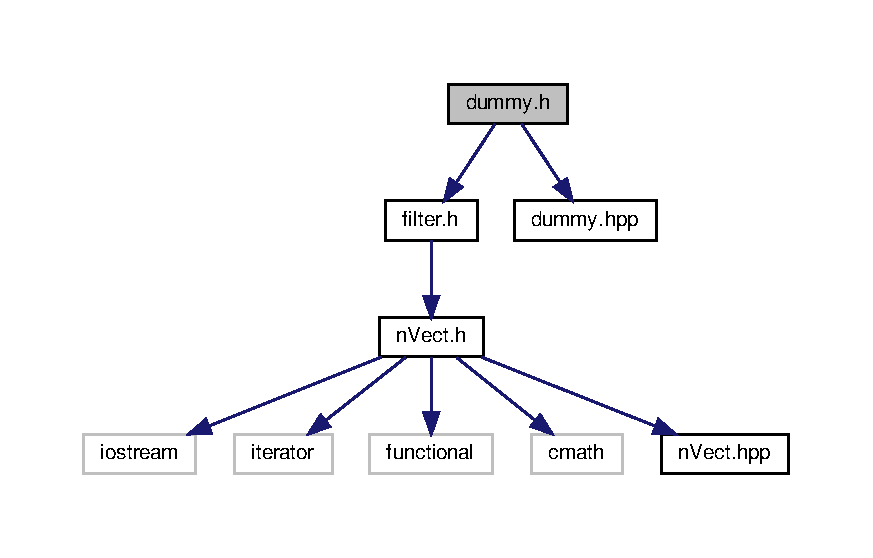
\includegraphics[width=350pt]{dummy_8h__incl}
\end{center}
\end{figure}
\subsection*{Classes}
\begin{DoxyCompactItemize}
\item 
class \hyperlink{classdummy}{dummy$<$ T $>$}
\begin{DoxyCompactList}\small\item\em dummy class. \end{DoxyCompactList}\end{DoxyCompactItemize}


\subsection{Detailed Description}
Definitions for the dummy filter derived class. ~\newline
Programmer\+: Noah Klein ~\newline
Class\+: C\+S5201 ~\newline
Assignment\+: Homework 5 ~\newline

\hypertarget{filter_8h}{}\section{filter.\+h File Reference}
\label{filter_8h}\index{filter.\+h@{filter.\+h}}
{\ttfamily \#include \char`\"{}n\+Vect.\+h\char`\"{}}\newline
Include dependency graph for filter.\+h\+:\nopagebreak
\begin{figure}[H]
\begin{center}
\leavevmode
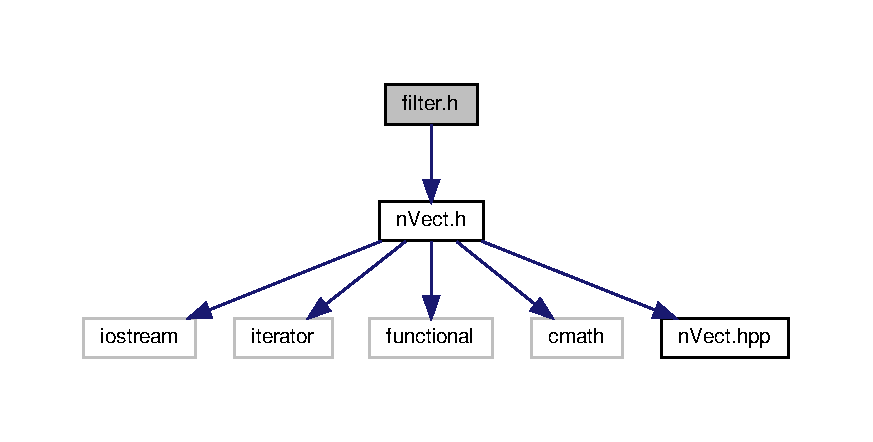
\includegraphics[width=350pt]{filter_8h__incl}
\end{center}
\end{figure}
This graph shows which files directly or indirectly include this file\+:\nopagebreak
\begin{figure}[H]
\begin{center}
\leavevmode
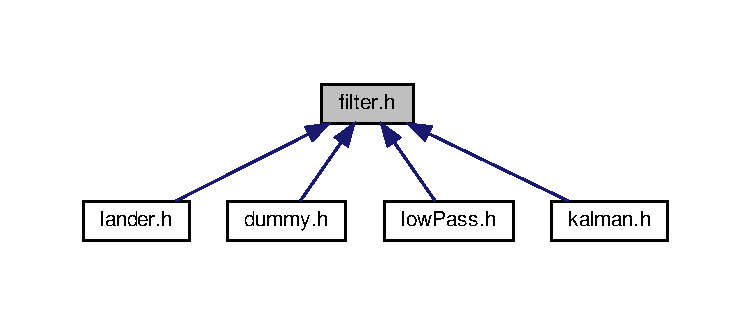
\includegraphics[width=350pt]{filter_8h__dep__incl}
\end{center}
\end{figure}
\subsection*{Classes}
\begin{DoxyCompactItemize}
\item 
class \hyperlink{classfilter}{filter$<$ T $>$}
\begin{DoxyCompactList}\small\item\em filter class. \end{DoxyCompactList}\end{DoxyCompactItemize}


\subsection{Detailed Description}
Definitions for the filter base class. ~\newline
Programmer\+: Noah Klein ~\newline
Class\+: C\+S5201 ~\newline
Assignment\+: Homework 5 ~\newline

\hypertarget{kalman_8h}{}\section{kalman.\+h File Reference}
\label{kalman_8h}\index{kalman.\+h@{kalman.\+h}}
{\ttfamily \#include \char`\"{}filter.\+h\char`\"{}}\newline
{\ttfamily \#include \char`\"{}kalman.\+hpp\char`\"{}}\newline
Include dependency graph for kalman.\+h\+:\nopagebreak
\begin{figure}[H]
\begin{center}
\leavevmode
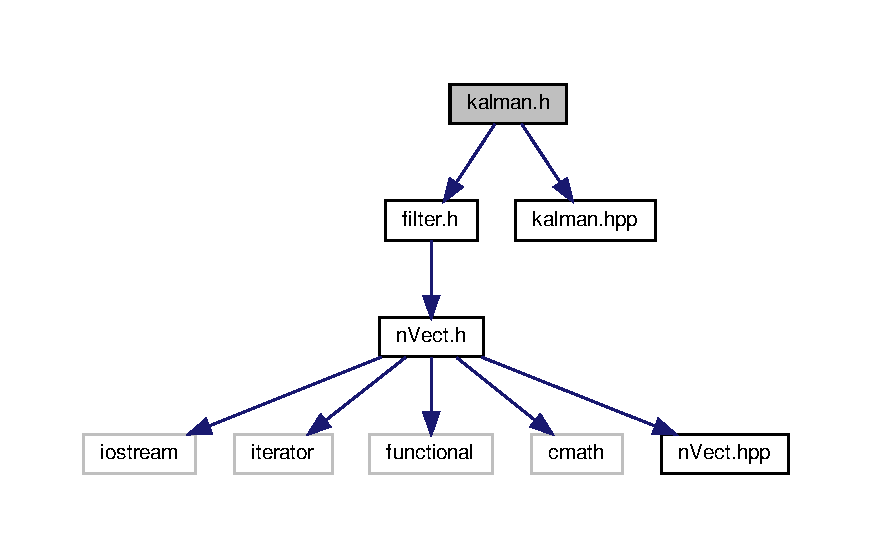
\includegraphics[width=350pt]{kalman_8h__incl}
\end{center}
\end{figure}
\subsection*{Classes}
\begin{DoxyCompactItemize}
\item 
class \hyperlink{classkalman}{kalman$<$ T $>$}
\begin{DoxyCompactList}\small\item\em kalman class. \end{DoxyCompactList}\end{DoxyCompactItemize}


\subsection{Detailed Description}
Definitions for the kalman filter derived class. ~\newline
Programmer\+: Noah Klein ~\newline
Class\+: C\+S5201 ~\newline
Assignment\+: Homework 5 ~\newline

\hypertarget{lander_8h}{}\section{lander.\+h File Reference}
\label{lander_8h}\index{lander.\+h@{lander.\+h}}
{\ttfamily \#include \char`\"{}n\+Vect.\+h\char`\"{}}\newline
{\ttfamily \#include \char`\"{}P\+I\+D.\+h\char`\"{}}\newline
{\ttfamily \#include \char`\"{}filter.\+h\char`\"{}}\newline
{\ttfamily \#include \char`\"{}lander.\+hpp\char`\"{}}\newline
Include dependency graph for lander.\+h\+:\nopagebreak
\begin{figure}[H]
\begin{center}
\leavevmode
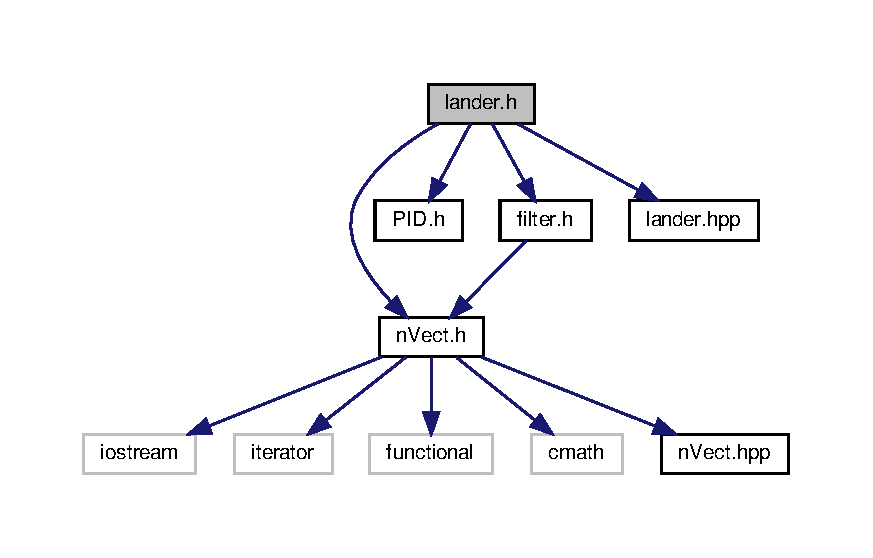
\includegraphics[width=350pt]{lander_8h__incl}
\end{center}
\end{figure}
\subsection*{Classes}
\begin{DoxyCompactItemize}
\item 
class \hyperlink{classlander}{lander}
\begin{DoxyCompactList}\small\item\em lander class. \end{DoxyCompactList}\end{DoxyCompactItemize}
\subsection*{Functions}
\begin{DoxyCompactItemize}
\item 
std\+::ostream \& \hyperlink{lander_8h_ab6f8c74d299fffd0364da0d38b9a8509}{operator$<$$<$} (std\+::ostream \&out, const \hyperlink{classlander}{lander} \&rhs)
\begin{DoxyCompactList}\small\item\em $<$$<$ operator \end{DoxyCompactList}\end{DoxyCompactItemize}


\subsection{Detailed Description}
Definitions for the lander class. ~\newline
Programmer\+: Noah Klein ~\newline
Class\+: C\+S5201 ~\newline
Assignment\+: Homework 5 ~\newline


\subsection{Function Documentation}
\mbox{\Hypertarget{lander_8h_ab6f8c74d299fffd0364da0d38b9a8509}\label{lander_8h_ab6f8c74d299fffd0364da0d38b9a8509}} 
\index{lander.\+h@{lander.\+h}!operator$<$$<$@{operator$<$$<$}}
\index{operator$<$$<$@{operator$<$$<$}!lander.\+h@{lander.\+h}}
\subsubsection{\texorpdfstring{operator$<$$<$()}{operator<<()}}
{\footnotesize\ttfamily std\+::ostream\& operator$<$$<$ (\begin{DoxyParamCaption}\item[{std\+::ostream \&}]{out,  }\item[{const \hyperlink{classlander}{lander} \&}]{rhs }\end{DoxyParamCaption})}



$<$$<$ operator 

Description\+: $<$$<$ operator overload for the lander class that allows the user to print the state information in a readable way. 
\begin{DoxyParams}{Parameters}
{\em out} & is the ostream object passed to the function. \\
\hline
{\em rhs} & is the lander object to be output to the user. \\
\hline
\end{DoxyParams}
\begin{DoxyReturn}{Returns}
Returns the ostream object. 
\end{DoxyReturn}
\begin{DoxyPostcond}{Postcondition}
The lander object is output to the user. 
\end{DoxyPostcond}

\hypertarget{lowPass_8h}{}\section{low\+Pass.\+h File Reference}
\label{lowPass_8h}\index{low\+Pass.\+h@{low\+Pass.\+h}}
{\ttfamily \#include \char`\"{}filter.\+h\char`\"{}}\newline
{\ttfamily \#include \char`\"{}low\+Pass.\+hpp\char`\"{}}\newline
Include dependency graph for low\+Pass.\+h\+:\nopagebreak
\begin{figure}[H]
\begin{center}
\leavevmode
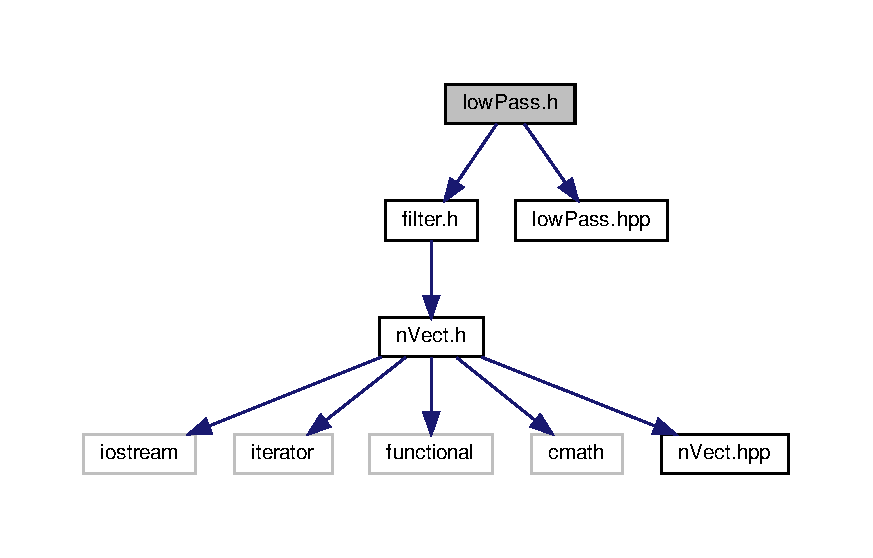
\includegraphics[width=350pt]{lowPass_8h__incl}
\end{center}
\end{figure}
\subsection*{Classes}
\begin{DoxyCompactItemize}
\item 
class \hyperlink{classlowPass}{low\+Pass$<$ T $>$}
\begin{DoxyCompactList}\small\item\em \hyperlink{classlowPass}{low\+Pass} class. \end{DoxyCompactList}\end{DoxyCompactItemize}


\subsection{Detailed Description}
Definitions for the lowpass filter derived class. ~\newline
Programmer\+: Noah Klein ~\newline
Class\+: C\+S5201 ~\newline
Assignment\+: Homework 5 ~\newline

\hypertarget{nTrix_8h}{}\section{n\+Trix.\+h File Reference}
\label{nTrix_8h}\index{n\+Trix.\+h@{n\+Trix.\+h}}
{\ttfamily \#include \char`\"{}n\+Vect.\+h\char`\"{}}\newline
{\ttfamily \#include \char`\"{}n\+Trix.\+hpp\char`\"{}}\newline
Include dependency graph for n\+Trix.\+h\+:\nopagebreak
\begin{figure}[H]
\begin{center}
\leavevmode
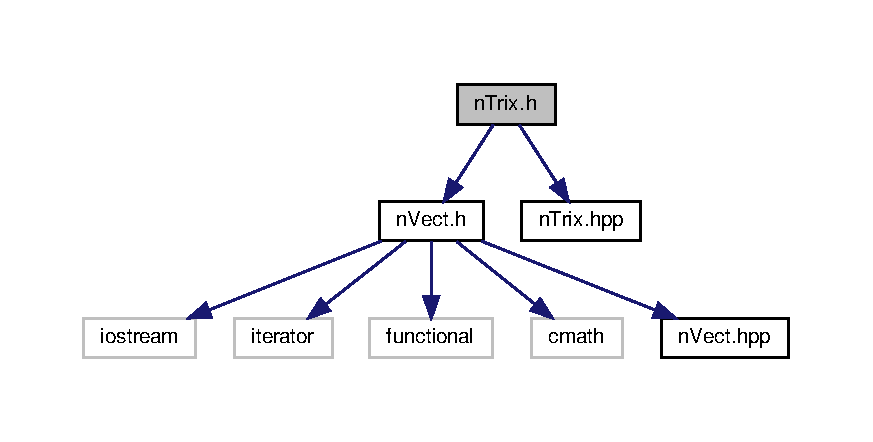
\includegraphics[width=350pt]{nTrix_8h__incl}
\end{center}
\end{figure}
\subsection*{Classes}
\begin{DoxyCompactItemize}
\item 
class \hyperlink{classnTrix}{n\+Trix$<$ T $>$}
\begin{DoxyCompactList}\small\item\em \hyperlink{classnTrix}{n\+Trix} class. \end{DoxyCompactList}\end{DoxyCompactItemize}
\subsection*{Functions}
\begin{DoxyCompactItemize}
\item 
{\footnotesize template$<$typename T $>$ }\\std\+::ostream \& \hyperlink{nTrix_8h_a2bbb75cad63d3ba6e6f96960e09a58e2}{operator$<$$<$} (std\+::ostream \&out, const \hyperlink{classnTrix}{n\+Trix}$<$ T $>$ \&rhs)
\begin{DoxyCompactList}\small\item\em $<$$<$ operator \end{DoxyCompactList}\item 
{\footnotesize template$<$typename T $>$ }\\std\+::istream \& \hyperlink{nTrix_8h_ad36b0a966daad207c03f790ace312827}{operator$>$$>$} (std\+::istream \&in, \hyperlink{classnTrix}{n\+Trix}$<$ T $>$ \&rhs)
\begin{DoxyCompactList}\small\item\em \begin{quote}
\begin{quote}
operator\end{quote}
\end{quote}
\end{DoxyCompactList}\item 
{\footnotesize template$<$typename T $>$ }\\\hyperlink{classnTrix}{n\+Trix}$<$ T $>$ \hyperlink{nTrix_8h_aa6a9cd47a847b2f5567e13bd6c9c1fac}{operator$\ast$} (const \hyperlink{classnTrix}{n\+Trix}$<$ T $>$ \&lhs, const float scalar)
\begin{DoxyCompactList}\small\item\em 
\begin{DoxyItemize}
\item operator 
\end{DoxyItemize}\end{DoxyCompactList}\item 
{\footnotesize template$<$typename T $>$ }\\\hyperlink{classnTrix}{n\+Trix}$<$ T $>$ \hyperlink{nTrix_8h_abdb8062a93fea20839bdf926b1e16f94}{operator$\ast$} (const \hyperlink{classnVect}{n\+Vect}$<$ T $>$ \&lhs, const \hyperlink{classnTrix}{n\+Trix}$<$ T $>$ \&rhs)
\begin{DoxyCompactList}\small\item\em 
\begin{DoxyItemize}
\item operator 
\end{DoxyItemize}\end{DoxyCompactList}\item 
{\footnotesize template$<$typename T $>$ }\\\hyperlink{classnTrix}{n\+Trix}$<$ float $>$ \hyperlink{nTrix_8h_acb6ffe9fd3e8aa373a570884247ac35b}{r\+\_\+invert} (const \hyperlink{classnTrix}{n\+Trix}$<$ T $>$ \&A, \hyperlink{classnTrix}{n\+Trix}$<$ float $>$ \&B, \hyperlink{classnTrix}{n\+Trix}$<$ float $>$ \&E, const \hyperlink{classnTrix}{n\+Trix}$<$ float $>$ \&I, float Cerror, float Perror)
\begin{DoxyCompactList}\small\item\em recursive invert \end{DoxyCompactList}\end{DoxyCompactItemize}


\subsection{Detailed Description}
Definitions for the \hyperlink{classnTrix}{n\+Trix} class. ~\newline
Programmer\+: Noah Klein ~\newline
Class\+: C\+S5201 ~\newline
Assignment\+: Homework 5 ~\newline


\subsection{Function Documentation}
\mbox{\Hypertarget{nTrix_8h_aa6a9cd47a847b2f5567e13bd6c9c1fac}\label{nTrix_8h_aa6a9cd47a847b2f5567e13bd6c9c1fac}} 
\index{n\+Trix.\+h@{n\+Trix.\+h}!operator$\ast$@{operator$\ast$}}
\index{operator$\ast$@{operator$\ast$}!n\+Trix.\+h@{n\+Trix.\+h}}
\subsubsection{\texorpdfstring{operator$\ast$()}{operator*()}\hspace{0.1cm}{\footnotesize\ttfamily [1/2]}}
{\footnotesize\ttfamily template$<$typename T $>$ \\
\hyperlink{classnTrix}{n\+Trix}$<$T$>$ operator$\ast$ (\begin{DoxyParamCaption}\item[{const \hyperlink{classnTrix}{n\+Trix}$<$ T $>$ \&}]{lhs,  }\item[{const float}]{scalar }\end{DoxyParamCaption})}




\begin{DoxyItemize}
\item operator 
\end{DoxyItemize}

Description\+: Scalar multiplication for a n\+Trix$<$\+T$>$ object. 
\begin{DoxyParams}{Parameters}
{\em lhs} & is the n\+Trix$<$\+T$>$ object to be multiplied through. \\
\hline
{\em scalar} & is the scalar to multiply through the matrix. \\
\hline
\end{DoxyParams}
\begin{DoxyReturn}{Returns}
Returns a new n\+Trix$<$\+T$>$ object with the scalar multiplied throughout. 
\end{DoxyReturn}
\begin{DoxyPrecond}{Precondition}
$\ast$ operator must be defined for type T. 
\end{DoxyPrecond}
\mbox{\Hypertarget{nTrix_8h_abdb8062a93fea20839bdf926b1e16f94}\label{nTrix_8h_abdb8062a93fea20839bdf926b1e16f94}} 
\index{n\+Trix.\+h@{n\+Trix.\+h}!operator$\ast$@{operator$\ast$}}
\index{operator$\ast$@{operator$\ast$}!n\+Trix.\+h@{n\+Trix.\+h}}
\subsubsection{\texorpdfstring{operator$\ast$()}{operator*()}\hspace{0.1cm}{\footnotesize\ttfamily [2/2]}}
{\footnotesize\ttfamily template$<$typename T $>$ \\
\hyperlink{classnTrix}{n\+Trix}$<$T$>$ operator$\ast$ (\begin{DoxyParamCaption}\item[{const \hyperlink{classnVect}{n\+Vect}$<$ T $>$ \&}]{lhs,  }\item[{const \hyperlink{classnTrix}{n\+Trix}$<$ T $>$ \&}]{rhs }\end{DoxyParamCaption})}




\begin{DoxyItemize}
\item operator 
\end{DoxyItemize}

Description\+: $\ast$ operator overload for the \hyperlink{classnTrix}{n\+Trix} class that allows the user to multiply a matrix with a vector. 
\begin{DoxyParams}{Parameters}
{\em lhs} & is a \hyperlink{classnVect}{n\+Vect} object to be multiplied to a \hyperlink{classnTrix}{n\+Trix}. \\
\hline
{\em rhs} & is a \hyperlink{classnTrix}{n\+Trix} object to be multiplied to a \hyperlink{classnVect}{n\+Vect}. \\
\hline
\end{DoxyParams}
\begin{DoxyReturn}{Returns}
Returns a n\+Trix$<$\+T$>$ object with the proper dimensions and with the values having matrix multiplicaion applied. 
\end{DoxyReturn}
\begin{DoxyPrecond}{Precondition}
$\ast$ operator must be defined for type T. 
\end{DoxyPrecond}

\begin{DoxyExceptions}{Exceptions}
{\em Throws} & a std\+::invalid\+\_\+argument object if the two matrices are not the correct dimensions for matrix multiplication to occur. \\
\hline
\end{DoxyExceptions}
\mbox{\Hypertarget{nTrix_8h_a2bbb75cad63d3ba6e6f96960e09a58e2}\label{nTrix_8h_a2bbb75cad63d3ba6e6f96960e09a58e2}} 
\index{n\+Trix.\+h@{n\+Trix.\+h}!operator$<$$<$@{operator$<$$<$}}
\index{operator$<$$<$@{operator$<$$<$}!n\+Trix.\+h@{n\+Trix.\+h}}
\subsubsection{\texorpdfstring{operator$<$$<$()}{operator<<()}}
{\footnotesize\ttfamily template$<$typename T $>$ \\
std\+::ostream\& operator$<$$<$ (\begin{DoxyParamCaption}\item[{std\+::ostream \&}]{out,  }\item[{const \hyperlink{classnTrix}{n\+Trix}$<$ T $>$ \&}]{rhs }\end{DoxyParamCaption})}



$<$$<$ operator 

Description\+: $<$$<$ operator overloaded to pretty print the \hyperlink{classnTrix}{n\+Trix} object. 
\begin{DoxyParams}{Parameters}
{\em out} & is the ostream object passed to the function. \\
\hline
{\em rhs} & is the n\+Trix$<$\+T$>$ object to be output. \\
\hline
\end{DoxyParams}
\begin{DoxyReturn}{Returns}
Returns the ostream. 
\end{DoxyReturn}
\begin{DoxyPrecond}{Precondition}
$<$$<$ operator must be defined for type T. 
\end{DoxyPrecond}
\begin{DoxyPostcond}{Postcondition}
Outputs the matrix to the user. 
\end{DoxyPostcond}
\mbox{\Hypertarget{nTrix_8h_ad36b0a966daad207c03f790ace312827}\label{nTrix_8h_ad36b0a966daad207c03f790ace312827}} 
\index{n\+Trix.\+h@{n\+Trix.\+h}!operator$>$$>$@{operator$>$$>$}}
\index{operator$>$$>$@{operator$>$$>$}!n\+Trix.\+h@{n\+Trix.\+h}}
\subsubsection{\texorpdfstring{operator$>$$>$()}{operator>>()}}
{\footnotesize\ttfamily template$<$typename T $>$ \\
std\+::istream\& operator$>$$>$ (\begin{DoxyParamCaption}\item[{std\+::istream \&}]{in,  }\item[{\hyperlink{classnTrix}{n\+Trix}$<$ T $>$ \&}]{rhs }\end{DoxyParamCaption})}



\begin{quote}
\begin{quote}
operator\end{quote}
\end{quote}


Description\+: $>$$>$ operator overloaded to extract a matrix object from the istream. The inputted matrix overloads any previously stored data in the \hyperlink{classnTrix}{n\+Trix} object. 
\begin{DoxyParams}{Parameters}
{\em in} & is the istream object passed to the function. \\
\hline
{\em rhs} & is the n\+Trix$<$\+T$>$ object to store the input. \\
\hline
\end{DoxyParams}
\begin{DoxyReturn}{Returns}
Returns the istream. 
\end{DoxyReturn}
\begin{DoxyPrecond}{Precondition}
$>$$>$ operator must be defined for type T. 
\end{DoxyPrecond}
\begin{DoxyPostcond}{Postcondition}
Stores the input in the object passed. 
\end{DoxyPostcond}

\begin{DoxyExceptions}{Exceptions}
{\em Throws} & a std\+::range\+\_\+error object if the user inputs an incorrect number of items for a column. \\
\hline
\end{DoxyExceptions}
\mbox{\Hypertarget{nTrix_8h_acb6ffe9fd3e8aa373a570884247ac35b}\label{nTrix_8h_acb6ffe9fd3e8aa373a570884247ac35b}} 
\index{n\+Trix.\+h@{n\+Trix.\+h}!r\+\_\+invert@{r\+\_\+invert}}
\index{r\+\_\+invert@{r\+\_\+invert}!n\+Trix.\+h@{n\+Trix.\+h}}
\subsubsection{\texorpdfstring{r\+\_\+invert()}{r\_invert()}}
{\footnotesize\ttfamily template$<$typename T $>$ \\
\hyperlink{classnTrix}{n\+Trix}$<$float$>$ r\+\_\+invert (\begin{DoxyParamCaption}\item[{const \hyperlink{classnTrix}{n\+Trix}$<$ T $>$ \&}]{A,  }\item[{\hyperlink{classnTrix}{n\+Trix}$<$ float $>$ \&}]{B,  }\item[{\hyperlink{classnTrix}{n\+Trix}$<$ float $>$ \&}]{E,  }\item[{const \hyperlink{classnTrix}{n\+Trix}$<$ float $>$ \&}]{I,  }\item[{float}]{Cerror,  }\item[{float}]{Perror }\end{DoxyParamCaption})}



recursive invert 

Description\+: Recursive part of the invert function that iteratively calculates the inverse of a matrix. 
\begin{DoxyParams}{Parameters}
{\em A} & is the matrix that the user wants the inverse of. \\
\hline
{\em B} & is the previous version of one of the matrices needed in the iterative calculation. \\
\hline
{\em E} & is one of the matrices needed in the iterative calculation. \\
\hline
{\em I} & is the identity matrix in the proper dimension of the matrix A. \\
\hline
{\em Cerror} & is the current frobenius norm of matrix B. \\
\hline
{\em Perror} & is the previous frobenius norm of matrix B. \\
\hline
\end{DoxyParams}
\begin{DoxyReturn}{Returns}
Returns an inverted matrix A. 
\end{DoxyReturn}
\begin{DoxyPrecond}{Precondition}
=, -\/, and $\ast$ operators need to be defined for type T. 
\end{DoxyPrecond}

\hypertarget{nVect_8h}{}\section{n\+Vect.\+h File Reference}
\label{nVect_8h}\index{n\+Vect.\+h@{n\+Vect.\+h}}
{\ttfamily \#include $<$iostream$>$}\newline
{\ttfamily \#include $<$iterator$>$}\newline
{\ttfamily \#include $<$functional$>$}\newline
{\ttfamily \#include $<$cmath$>$}\newline
{\ttfamily \#include \char`\"{}n\+Vect.\+hpp\char`\"{}}\newline
Include dependency graph for n\+Vect.\+h\+:\nopagebreak
\begin{figure}[H]
\begin{center}
\leavevmode
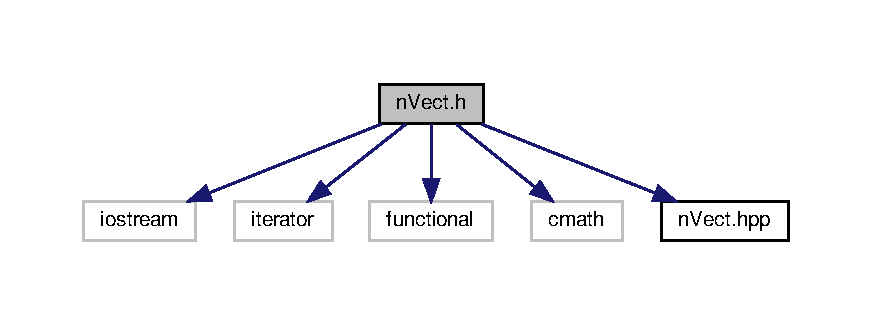
\includegraphics[width=350pt]{nVect_8h__incl}
\end{center}
\end{figure}
This graph shows which files directly or indirectly include this file\+:\nopagebreak
\begin{figure}[H]
\begin{center}
\leavevmode
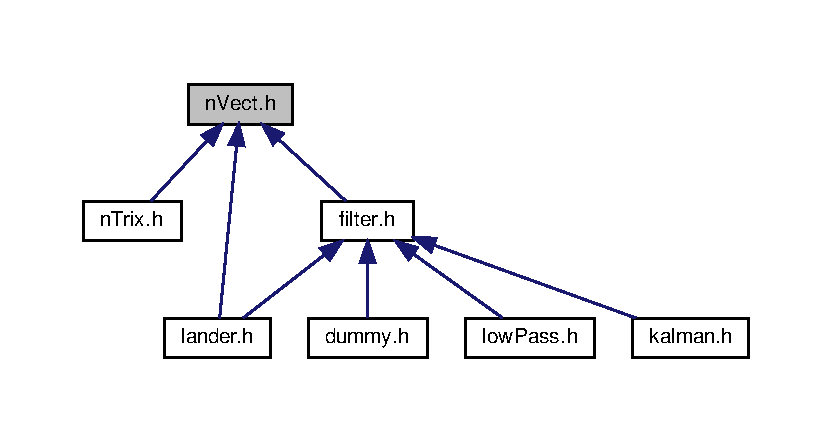
\includegraphics[width=350pt]{nVect_8h__dep__incl}
\end{center}
\end{figure}
\subsection*{Classes}
\begin{DoxyCompactItemize}
\item 
class \hyperlink{classnVect}{n\+Vect$<$ T $>$}
\begin{DoxyCompactList}\small\item\em \hyperlink{classnVect}{n\+Vect} class. \end{DoxyCompactList}\item 
class \hyperlink{classnVect_1_1iterator}{n\+Vect$<$ T $>$\+::iterator}
\begin{DoxyCompactList}\small\item\em iterator class. \end{DoxyCompactList}\end{DoxyCompactItemize}
\subsection*{Functions}
\begin{DoxyCompactItemize}
\item 
{\footnotesize template$<$typename T $>$ }\\\hyperlink{classnVect}{n\+Vect}$<$ T $>$ \hyperlink{nVect_8h_aaea4ae2e2f0c095902f38c22928c9d31}{operator+} (const \hyperlink{classnVect}{n\+Vect}$<$ T $>$ \&lhs, const \hyperlink{classnVect}{n\+Vect}$<$ T $>$ \&rhs)
\begin{DoxyCompactList}\small\item\em 
\begin{DoxyItemize}
\item operator 
\end{DoxyItemize}\end{DoxyCompactList}\item 
{\footnotesize template$<$typename T $>$ }\\\hyperlink{classnVect}{n\+Vect}$<$ T $>$ \hyperlink{nVect_8h_a8b1ac989f8040b056775eaeb81c506d2}{operator$\ast$} (const \hyperlink{classnVect}{n\+Vect}$<$ T $>$ \&lhs, const T \&rhs)
\begin{DoxyCompactList}\small\item\em Scalar multiplication. \end{DoxyCompactList}\item 
{\footnotesize template$<$typename T $>$ }\\\hyperlink{classnVect}{n\+Vect}$<$ T $>$ \hyperlink{nVect_8h_ab14d927799a17a9ecdaec6471fe51079}{operator$\ast$} (const T \&lhs, const \hyperlink{classnVect}{n\+Vect}$<$ T $>$ \&rhs)
\begin{DoxyCompactList}\small\item\em Scalar multiplication. \end{DoxyCompactList}\item 
{\footnotesize template$<$typename T $>$ }\\std\+::ostream \& \hyperlink{nVect_8h_ac41f0d1072a4da1e6b7e1c0139d7edaa}{operator$<$$<$} (std\+::ostream \&out, const \hyperlink{classnVect}{n\+Vect}$<$ T $>$ \&rhs)
\begin{DoxyCompactList}\small\item\em $<$$<$ operator \end{DoxyCompactList}\item 
{\footnotesize template$<$typename T $>$ }\\std\+::istream \& \hyperlink{nVect_8h_a633c2e020b48c20b53f449795b64317d}{operator$>$$>$} (std\+::istream \&in, \hyperlink{classnVect}{n\+Vect}$<$ T $>$ \&rhs)
\begin{DoxyCompactList}\small\item\em \begin{quote}
\begin{quote}
operator\end{quote}
\end{quote}
\end{DoxyCompactList}\end{DoxyCompactItemize}


\subsection{Detailed Description}
Definitions for the \hyperlink{classnVect}{n\+Vect} class. ~\newline
Programmer\+: Noah Klein ~\newline
Class\+: C\+S5201 ~\newline
Assignment\+: Homework 5 ~\newline


\subsection{Function Documentation}
\mbox{\Hypertarget{nVect_8h_a8b1ac989f8040b056775eaeb81c506d2}\label{nVect_8h_a8b1ac989f8040b056775eaeb81c506d2}} 
\index{n\+Vect.\+h@{n\+Vect.\+h}!operator$\ast$@{operator$\ast$}}
\index{operator$\ast$@{operator$\ast$}!n\+Vect.\+h@{n\+Vect.\+h}}
\subsubsection{\texorpdfstring{operator$\ast$()}{operator*()}\hspace{0.1cm}{\footnotesize\ttfamily [1/2]}}
{\footnotesize\ttfamily template$<$typename T $>$ \\
\hyperlink{classnVect}{n\+Vect}$<$T$>$ operator$\ast$ (\begin{DoxyParamCaption}\item[{const \hyperlink{classnVect}{n\+Vect}$<$ T $>$ \&}]{lhs,  }\item[{const T \&}]{rhs }\end{DoxyParamCaption})}



Scalar multiplication. 

Description\+: Allows for scalar multiplication of a calling vector. 
\begin{DoxyParams}{Parameters}
{\em lhs} & is the \hyperlink{classnVect}{n\+Vect} that the scalar will be multiplied through. \\
\hline
{\em rhs} & is a scalar of type T to be multiplied through the vector. \\
\hline
\end{DoxyParams}
\begin{DoxyReturn}{Returns}
Returns a newly created vector where the data in each container has been multiplied by the scalar. 
\end{DoxyReturn}
\begin{DoxyPrecond}{Precondition}
$\ast$= operator needs to be defined for type T. 
\end{DoxyPrecond}
\begin{DoxyPostcond}{Postcondition}
Creates a new vector that gets returned. 
\end{DoxyPostcond}
\mbox{\Hypertarget{nVect_8h_ab14d927799a17a9ecdaec6471fe51079}\label{nVect_8h_ab14d927799a17a9ecdaec6471fe51079}} 
\index{n\+Vect.\+h@{n\+Vect.\+h}!operator$\ast$@{operator$\ast$}}
\index{operator$\ast$@{operator$\ast$}!n\+Vect.\+h@{n\+Vect.\+h}}
\subsubsection{\texorpdfstring{operator$\ast$()}{operator*()}\hspace{0.1cm}{\footnotesize\ttfamily [2/2]}}
{\footnotesize\ttfamily template$<$typename T $>$ \\
\hyperlink{classnVect}{n\+Vect}$<$T$>$ operator$\ast$ (\begin{DoxyParamCaption}\item[{const T \&}]{lhs,  }\item[{const \hyperlink{classnVect}{n\+Vect}$<$ T $>$ \&}]{rhs }\end{DoxyParamCaption})}



Scalar multiplication. 

Description\+: Allows for scalar multiplication of a calling vector. 
\begin{DoxyParams}{Parameters}
{\em lhs} & is a \hyperlink{classnVect}{n\+Vect} that the scalar will be muliplied through. \\
\hline
{\em rhs} & is a scalar of type T to be multiplied through the vector. \\
\hline
\end{DoxyParams}
\begin{DoxyReturn}{Returns}
Returns a newly created vector where the data in each container has been multiplied by the scalar. 
\end{DoxyReturn}
\begin{DoxyPrecond}{Precondition}
$\ast$= operator needs to be defined for type T. 
\end{DoxyPrecond}
\begin{DoxyPostcond}{Postcondition}
Creates a new vector that gets returned. 
\end{DoxyPostcond}
\mbox{\Hypertarget{nVect_8h_aaea4ae2e2f0c095902f38c22928c9d31}\label{nVect_8h_aaea4ae2e2f0c095902f38c22928c9d31}} 
\index{n\+Vect.\+h@{n\+Vect.\+h}!operator+@{operator+}}
\index{operator+@{operator+}!n\+Vect.\+h@{n\+Vect.\+h}}
\subsubsection{\texorpdfstring{operator+()}{operator+()}}
{\footnotesize\ttfamily template$<$typename T $>$ \\
\hyperlink{classnVect}{n\+Vect}$<$T$>$ operator+ (\begin{DoxyParamCaption}\item[{const \hyperlink{classnVect}{n\+Vect}$<$ T $>$ \&}]{lhs,  }\item[{const \hyperlink{classnVect}{n\+Vect}$<$ T $>$ \&}]{rhs }\end{DoxyParamCaption})}




\begin{DoxyItemize}
\item operator 
\end{DoxyItemize}

Description\+: Used to add two vectors together. Allows for vectors of different (or similar) sizes to be added through vector addition. 
\begin{DoxyParams}{Parameters}
{\em lhs} & is the \hyperlink{classnVect}{n\+Vect} to be added to. \\
\hline
{\em rhs} & is the \hyperlink{classnVect}{n\+Vect} to be added to the calling object. \\
\hline
\end{DoxyParams}
\begin{DoxyReturn}{Returns}
Returns a newly created vector where each container now holds the sum of the two vectors passed at that index. 
\end{DoxyReturn}
\begin{DoxyPrecond}{Precondition}
+= operator needs to be defined for type T. 
\end{DoxyPrecond}
\begin{DoxyPostcond}{Postcondition}
Creates a new vector that gets returned. 
\end{DoxyPostcond}
\mbox{\Hypertarget{nVect_8h_ac41f0d1072a4da1e6b7e1c0139d7edaa}\label{nVect_8h_ac41f0d1072a4da1e6b7e1c0139d7edaa}} 
\index{n\+Vect.\+h@{n\+Vect.\+h}!operator$<$$<$@{operator$<$$<$}}
\index{operator$<$$<$@{operator$<$$<$}!n\+Vect.\+h@{n\+Vect.\+h}}
\subsubsection{\texorpdfstring{operator$<$$<$()}{operator<<()}}
{\footnotesize\ttfamily template$<$typename T $>$ \\
std\+::ostream\& operator$<$$<$ (\begin{DoxyParamCaption}\item[{std\+::ostream \&}]{out,  }\item[{const \hyperlink{classnVect}{n\+Vect}$<$ T $>$ \&}]{rhs }\end{DoxyParamCaption})}



$<$$<$ operator 

Description\+: Allows for proper outputting of \hyperlink{classnVect}{n\+Vect} objects. 
\begin{DoxyParams}{Parameters}
{\em out} & is the ostream passed. \\
\hline
{\em rhs} & is the \hyperlink{classnVect}{n\+Vect} to be output. \\
\hline
\end{DoxyParams}
\begin{DoxyReturn}{Returns}
Returns the ostream 
\end{DoxyReturn}
\begin{DoxyPrecond}{Precondition}
$<$$<$ operator must be defined for type T. 
\end{DoxyPrecond}
\begin{DoxyPostcond}{Postcondition}
Outputs the object to the stream. 
\end{DoxyPostcond}
\mbox{\Hypertarget{nVect_8h_a633c2e020b48c20b53f449795b64317d}\label{nVect_8h_a633c2e020b48c20b53f449795b64317d}} 
\index{n\+Vect.\+h@{n\+Vect.\+h}!operator$>$$>$@{operator$>$$>$}}
\index{operator$>$$>$@{operator$>$$>$}!n\+Vect.\+h@{n\+Vect.\+h}}
\subsubsection{\texorpdfstring{operator$>$$>$()}{operator>>()}}
{\footnotesize\ttfamily template$<$typename T $>$ \\
std\+::istream\& operator$>$$>$ (\begin{DoxyParamCaption}\item[{std\+::istream \&}]{in,  }\item[{\hyperlink{classnVect}{n\+Vect}$<$ T $>$ \&}]{rhs }\end{DoxyParamCaption})}



\begin{quote}
\begin{quote}
operator\end{quote}
\end{quote}


Description\+: Allows the user to insert any amount of data into a \hyperlink{classnVect}{n\+Vect} object. 
\begin{DoxyParams}{Parameters}
{\em in} & is the istream passed. \\
\hline
{\em rhs} & is the \hyperlink{classnVect}{n\+Vect} to store input. \\
\hline
\end{DoxyParams}
\begin{DoxyReturn}{Returns}
Returns the istream. 
\end{DoxyReturn}
\begin{DoxyPostcond}{Postcondition}
Inputted data is stored in the rhs \hyperlink{classnVect}{n\+Vect}. 
\end{DoxyPostcond}

\hypertarget{PID_8h}{}\section{P\+I\+D.\+h File Reference}
\label{PID_8h}\index{P\+I\+D.\+h@{P\+I\+D.\+h}}
This graph shows which files directly or indirectly include this file\+:\nopagebreak
\begin{figure}[H]
\begin{center}
\leavevmode
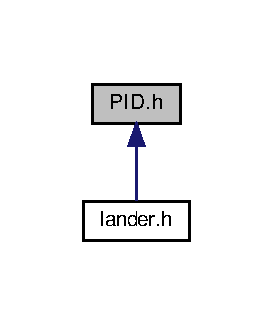
\includegraphics[width=131pt]{PID_8h__dep__incl}
\end{center}
\end{figure}
\subsection*{Classes}
\begin{DoxyCompactItemize}
\item 
class \hyperlink{classPID}{P\+ID}
\begin{DoxyCompactList}\small\item\em \hyperlink{classPID}{P\+ID} class. \end{DoxyCompactList}\end{DoxyCompactItemize}


\subsection{Detailed Description}
Definitions for the \hyperlink{classPID}{P\+ID} class. ~\newline
Programmer\+: Noah Klein ~\newline
Class\+: C\+S5201 ~\newline
Assignment\+: Homework 5 ~\newline

%--- End generated contents ---

% Index
\backmatter
\newpage
\phantomsection
\clearemptydoublepage
\addcontentsline{toc}{chapter}{Index}
\printindex

\end{document}
